\documentclass[11pt,a4paper,openany]{report}
\usepackage[utf8]{inputenc}
\usepackage[english]{babel}
\usepackage[T1]{fontenc}
\usepackage{amsmath}
\usepackage{amsfonts}
\usepackage{amssymb}
\usepackage{makeidx}
\usepackage{graphicx}
\usepackage{float}
\usepackage{lmodern}
\usepackage[dvipsnames]{xcolor}
\usepackage{tikz}
\usetikzlibrary{intersections}
\usepackage{pgfplots}
\usetikzlibrary{calc}
\usepackage{geometry}
\geometry{hmargin=2cm,vmargin=2cm}
\usepackage{fancybox}
\usepackage{mathtools}
\usepackage{enumitem}
\usepackage{tcolorbox}
\usepackage{colortbl}
\usepackage{fancybox}
\tcbuselibrary{most}
\usepackage{pifont}
\usepackage[skip = 5pt, font = {footnotesize}, labelfont = sl]{caption}
\usepackage{subcaption}
\usepackage{eso-pic}
\usepackage{nicematrix}
\usepackage{multicol}
\usepackage{booktabs}
\usepackage{svg}
\usepackage{derivative}
\usepackage{wrapfig}
\usepackage{stmaryrd}
\usepackage{yfonts}
\usepackage{array}
\usepackage{csquotes}
\usepackage[style=phys , backend=biber]{biblatex}
\addbibresource{bibliography.bib}
\author{Andrea}
\setlength{\columnsep}{.5cm}
\usepackage{titlesec}
\usepackage{lipsum}
\usepackage{indentfirst}
\usepackage{tabularx}


% use Roman numerals for sections
\renewcommand{\thesection}{\Roman{section}}

% use Arabic numerals for subsections
\renewcommand{\thesubsection}{\arabic{subsection}}

% use letters for subsubsections with a parenthesis
\renewcommand{\thesubsubsection}{\alph{subsubsection})}

% put a period and space after numbers
\titlelabel{\thetitle\thickspace}

% Make section titles centered and bold
\titleformat*{\section}{\centering\bfseries}
\titleformat*{\subsection}{\bfseries}

% Make subsections centered and italc
 % Make subsubsections centered
\titleformat*{\subsubsection}{\centering}
\titleclass{\chapter}{straight}
\titleformat{\chapter}[frame]
{\normalfont}
{\filright
\footnotesize
\enspace \texttt{CHAPTER \thechapter} \enspace}
{8pt}
{\Large\bfseries\filcenter}

\titlespacing*{\chapter}{0pt}{10pt}{10pt}
\titlespacing{\section}{0pt}{*3}{*3}
\titlespacing{\subsection}{0pt}{*1.5}{*1.5}
\titlespacing{\subsubsection}{0pt}{*1.5}{*1.5}


\usepackage{amsmath}
\colorlet{shadecolor}{cyan!15}
\usepackage{fancyhdr}
\usepackage{etoolbox}
\usepackage[export]{adjustbox}
\usepackage{fourier-orns}
\usepackage{lettrine}
\usepackage{physics}
\usepackage{hyperref}
\usepackage{titlesec}
\usepackage[titletoc]{appendix}
\usepackage{adforn}
\hypersetup{
    colorlinks=false,
    linkbordercolor = {white},
    menubordercolor = {white},
    citebordercolor = {black},
    urlbordercolor = {black},
}
\captionsetup{singlelinecheck=off, box=colorbox,boxcolor=gray!15, labelsep=endash}

\definecolor{RoyalRed}{RGB}{157,16, 45}
\pgfmathdeclarefunction{gauss}{2}{%
  \pgfmathparse{1/(#2*sqrt(2*pi))*exp(-((x-#1)^2)/(2*#2^2))}%
}
\usetikzlibrary{decorations.markings}
\renewcommand{\headrule}{%
\vspace{6pt}\hrulefill
\raisebox{0pt}{\quad\adforn{64} \adforn{8} \adforn{36}\quad}\hrulefill}
\pagestyle{fancy}
\fancyhf{}
\rhead{ \textcolor{black}{\footnotesize \today}}
\lhead{ENS}
\chead{ \textcolor{black}{· \emph{\leftmark} ·}}
\rfoot{Andrea Combette}
\fancyfoot[C]{\thepage}

\newlength{\tabcont}


\setcounter{tocdepth}{4}
\setcounter{secnumdepth}{4}

\begin{document}
\begin{titlepage}
    \AddToShipoutPictureBG*{
        \begin{tikzpicture}[overlay,remember picture]
            \draw [line width=3pt]
            ($ (current page.north west) + (2cm,-2.0cm) $)
            rectangle
            ($ (current page.south east) + (-2cm,1.8cm) $);
            \draw [line width=1pt]
            ($ (current page.north west) + (2.15cm,-2.15cm) $)
            rectangle
            ($ (current page.south east) + (-2.15cm,1.95cm) $);
        \end{tikzpicture}
    }
    \begin{center}
        \vspace*{2cm}
        \emph{\footnotesize{Department of physics, École Normale Supérieure, Paris}}

        \emph{\footnotesize{Swiss Plasma Center, EPFL, Lausanne}}


        \vspace*{1cm}

        \textsc{Trapped Electron Mode}

        \textsc{Characterization by Short Pulse Reflectometry}
        \vspace*{1cm}

        \rule{14cm}{2pt}\vspace{.7cm}

        \Large{\textbf{Master Thesis 2024}}

        \vspace{.5cm}
        \rule{14cm}{2pt}
        \vspace{1cm}

        \Large Andrea Combette

        \vspace{3cm}

        \raisebox{-5pt}{\quad\decofourleft\decotwo\decofourright\quad}

        \vspace{2cm}
        \vspace{1cm}

        \begin{minipage}{14cm}
            \small{\textbf{Supervisors:}}
            \vspace{.5cm}

            \small{\textbf{Dr. Oleg Krutkin \null\hfill Pr. Jean François Allemand}}

        \end{minipage}
        \vspace{2cm}


        % \begin{minipage}{14cm}
        %     \small{
        %         \textbf{Cautionary note : } This paper is a report on numerical methods for the shallow water equations and gravity waves. It is not intended to be a complete and rigorous study of the subject. The reader is invited to refer to the references for further details.
        %         It has been made by a Master Student, with some background in physics and mathematics, but no prior knowledge of the subject. It is therefore not intended to be a reference for experts in the field.}
        % \end{minipage}

    \end{center}

\end{titlepage}

\newpage
\vspace*{2cm}
\renewcommand{\contentsname}{TABLE OF CONTENTS} % Rename ToC title

\begin{multicols}{2}
    \renewcommand{\baselinestretch}{1.7}\normalsize % Adjust spacing of ToC
    {\small \tableofcontents} % Set font size for ToC



    \renewcommand{\baselinestretch}{1.0}\normalsize

\end{multicols}
\newpage


\begin{center}
    \textbf{ABSTRACT}
\end{center}
\fontsize{9}{10}\selectfont

\lettrine[loversize=.30,findent=.21em,nindent=2.5pt]{\color{black} T}{he} \emph{ report is devoted
    to investigation of turbulence characteristics in the TCV tokamak using Short Pulse Reflectometry diagnostic and Machine Learning approach, focusing on Trapped Electron Mode (TEM) instabilities and their impact on radial transport. A 1D model initially provided insights, but a 2D model was developed to better account for curvature, incidence angle, and scattering effects. Using extensive CUWA code simulations, datasets were generated for both Gaussian and power spectrum turbulence structures accounting for various simulation parameters like the position of the cut-off the structures of turbulences \dots The 2D model achieved $R^2$ scores of 0.92 for Gaussian and 0.89 for power spectrum tests, outperforming deeper neural networks. It effectively managed non-linear effects, delay characteristics, and cut-off layer shifts.}
\fontsize{10}{10}\selectfont

\begin{multicols}{2}
    \chapter*{Introduction}
    \lettrine[loversize=.30,findent=.21em,nindent=2.5pt]{\color{black} O}{ne} of the common goal in experimental magnetically confined fusion research is the characterization of plasma turbulence. To achieve this, the TCV tokamak features a novel short-pulse reflectometry (SPR) diagnostic that can potentially measure the properties of this turbulence.
    The SPR diagnostic operates as a radar system. It probes the plasma with a very short microwave pulse (under one nanosecond), which reflects off the cutoff (reflection) region back into the probing antenna. The position of this cutoff, for probing frequencies in the range of 50-75 GHz, is determined by the plasma electron density. By measuring the time delay between the probing pulse and the reflected pulse at different frequencies, the electron density profile, including its turbulent perturbations, can be inferred.
    However, the complex interaction between microwaves and magnetized plasma makes it challenging to link SPR measurements with turbulence properties. Numerical modeling using a synthetic diagnostic approach has been performed for cases with low turbulence amplitudes (linear regime). The scenario with large turbulence amplitudes (nonlinear regime) remains unexplored.
    This project will conduct a systematic analysis of the SPR diagnostic in the nonlinear regime. The numerical finite difference code CUWA, which solves the wave equation for given plasma density and magnetic field and provides synthetic reflected pulses, will be used. The main objectives are to identify markers indicating whether the diagnostic is operating in the nonlinear regime and to assess the feasibility of determining turbulence parameters.
    \chapter{Theoretical Background}

    \section{Nuclear Fusion}
    \subsection{Fusion Reaction}
    \lettrine[lines=2, lhang=.3, nindent=0pt]{\color{black} T}{he} Nuclear fusion is the process by which two atomic nuclei combine to form a heavier nucleus. This process is accompanied by the release or absorption of energy, depending on the masses of the nuclei involved. Typically, lighter nuclei release more energy because the short-range nuclear force is overcome more easily for light nuclei.

    However, to overcome the Coulomb barrier, the nuclei must be brought close enough together for a long enough time to allow quantum tunneling to occur. To achieve this, the reactants must be heated to extremely high temperatures, ionizing them and turning them into plasma. It has been found that the probability of collision, or cross-section, is highest for the Deuterium-Tritium mixture.

    \begin{align*}
        \text{D}^2 + \text{T}^3 & \rightarrow \text{He}^4 + \text{n[17.6 MeV]}
    \end{align*}
    \subsection{Tokamak confinement}
    A key component of the fusion process is the duration for which the plasma can be effectively confined. This confinement can be achieved through various methods. One of the most promising and well-established approaches is the Tokamak vessel, which employs magnetic confinement to maintain the plasma in a toroidal shape. The plasma is heated to several million degrees, allowing the fusion reaction to be sustained. The energy released from the fusion reaction is used both to heat the plasma and to sustain the reaction.

    The energy balance in a Tokamak is governed by the Lawson criterion, which compares the energy confinement time to the energy loss time. The energy confinement time depends on the plasma density and temperature, while the energy loss time is determined by the plasma's losses.
    $$n \tau E \ge 1.5.10^{20}{\frac {\mathrm {s} }{\mathrm {m} ^{3}}}$$
    \begin{figure}[H]
        \centering
        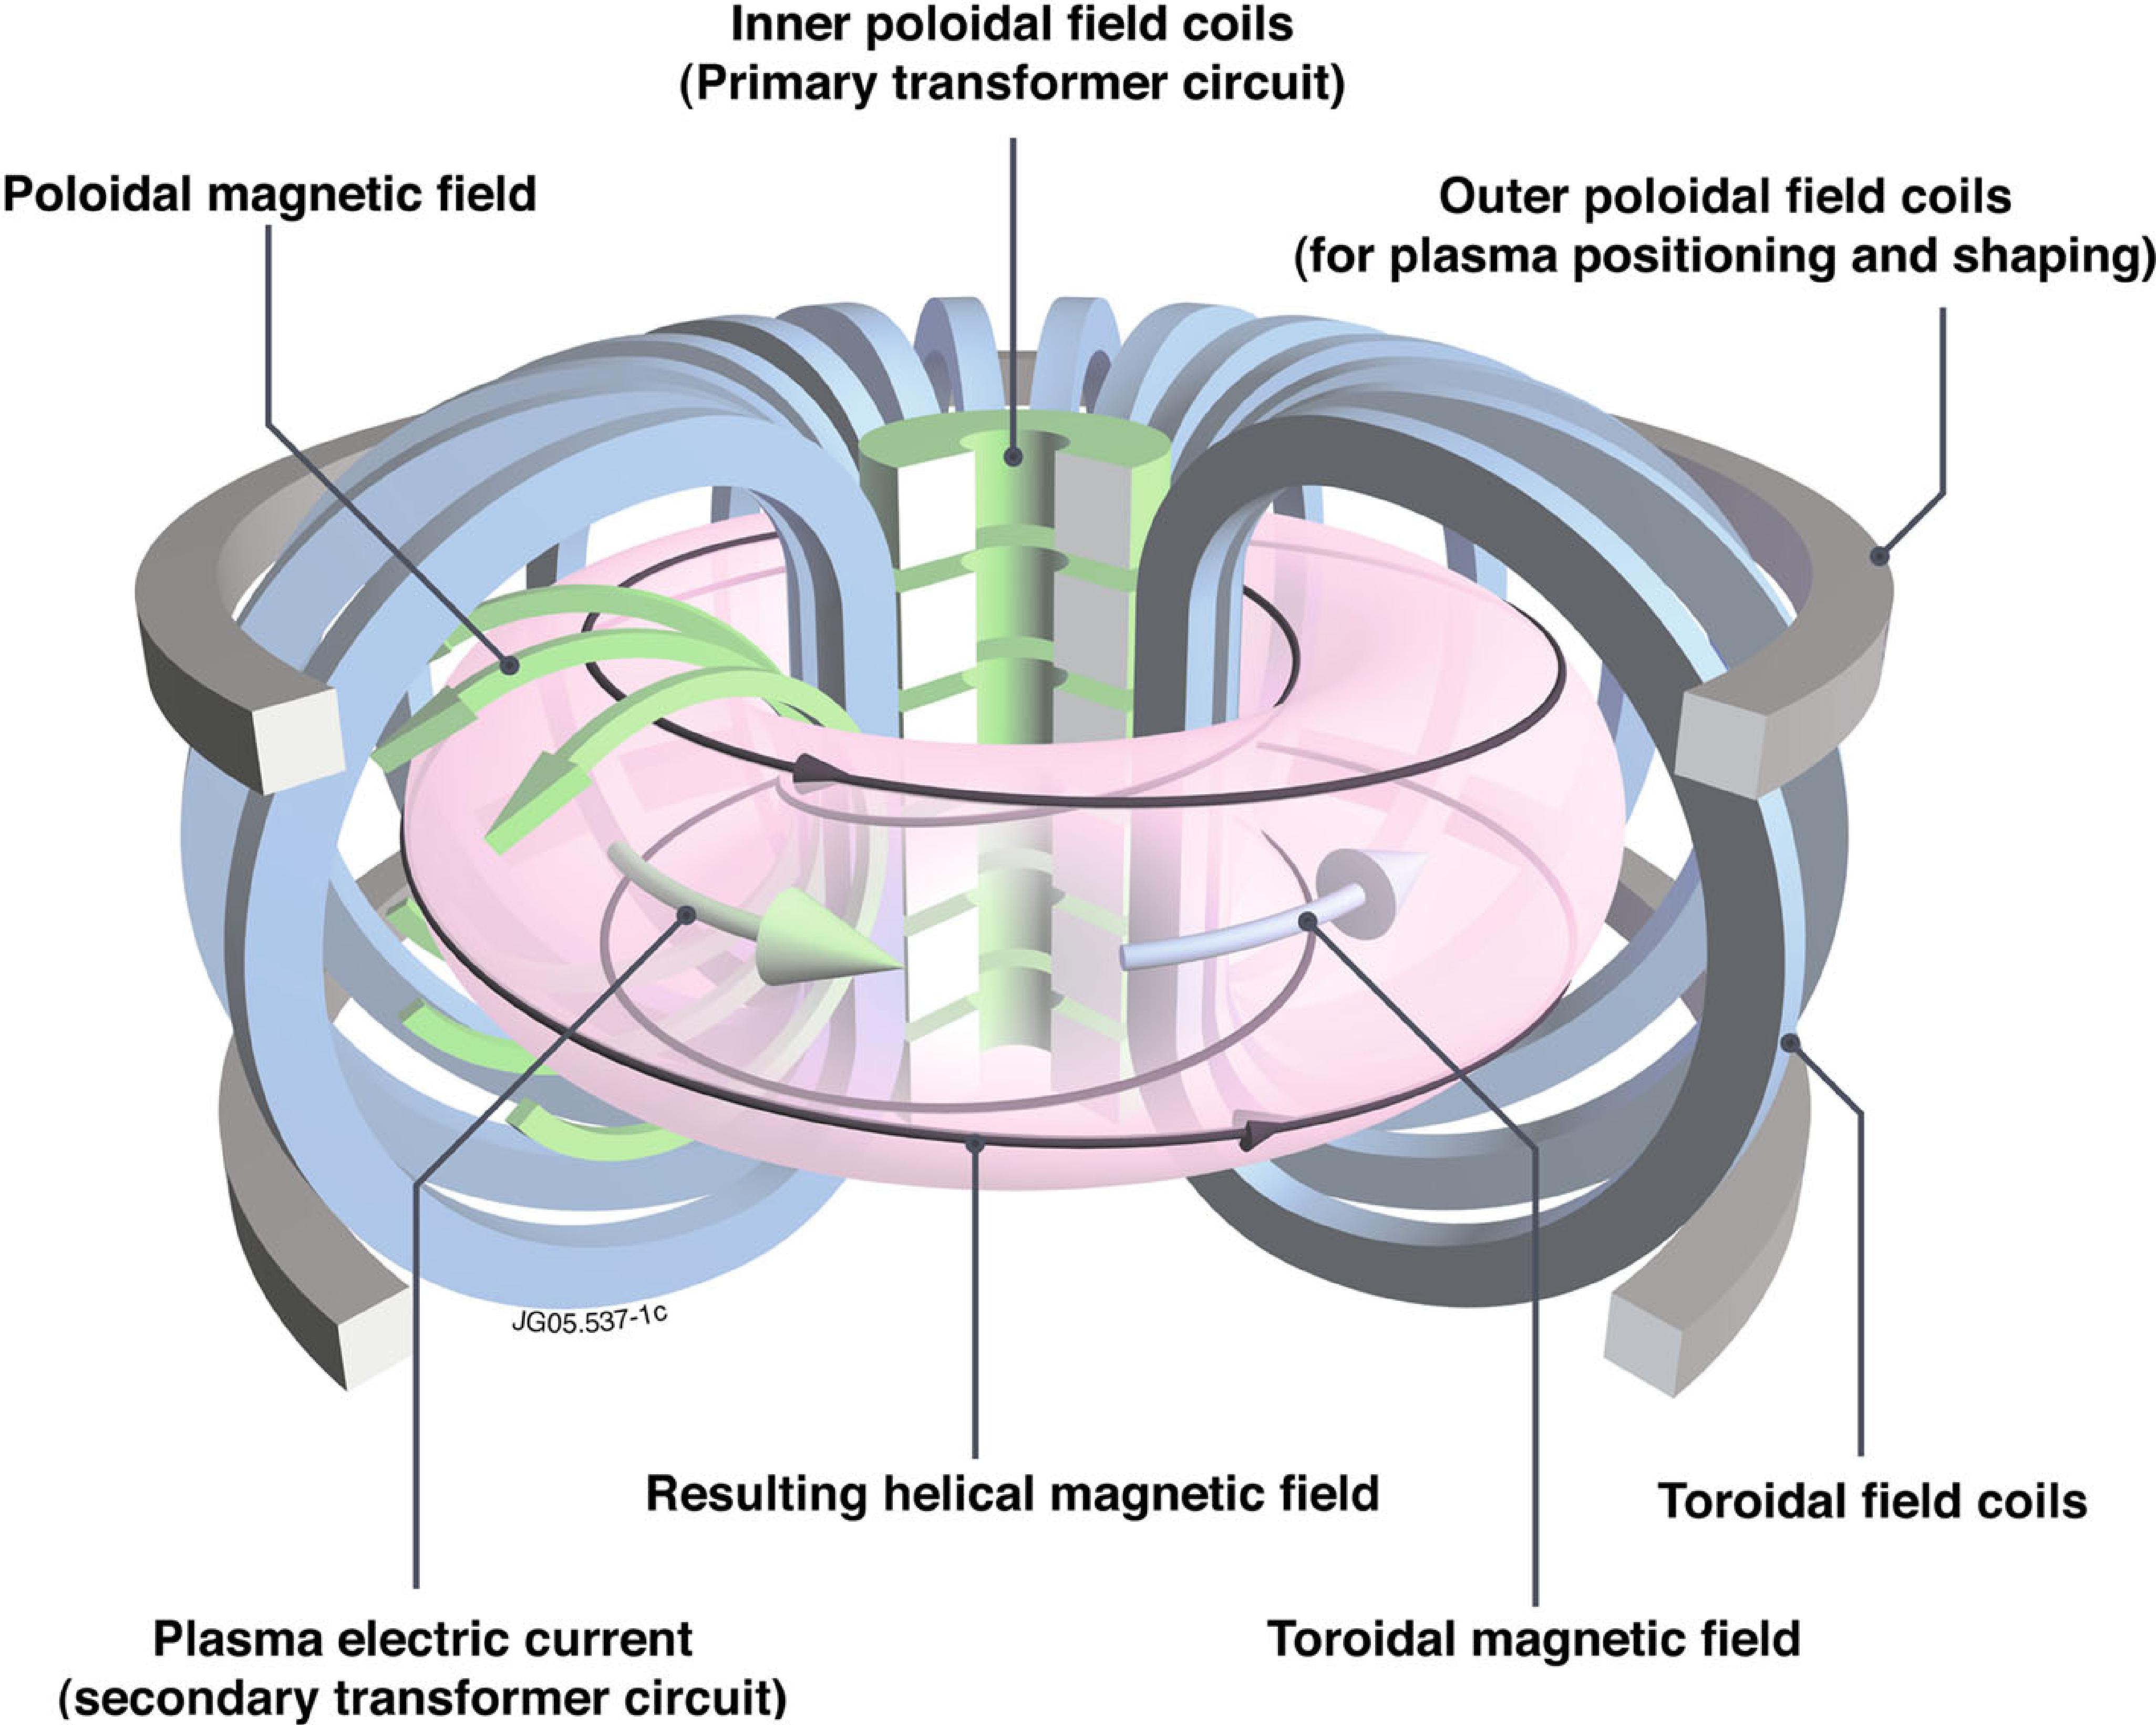
\includegraphics[width=1\linewidth]{./figures/tokamak.png}
        \caption{Simplification of Tokamak device, the toroidal magnetic field is generated by coils, while the poloidal magnetic field is produced by the plasma current and poloidal field coils. The plasma is heated by various devices, enabling the fusion reaction to be sustained.}
        \label{}
    \end{figure}
    This confinement is realized by applying a strong magnetic field in the toroidal direction. The magnetic field is generated by a set of coils, which are arranged in a toroidal shape, and the plasma is heated by various methods \cite{Heating}. The neoclassical geometries in the Tokamak lead to several physical phenomena such as charge separation in the Tokamak, drift kinetics, and turbulence. The curvature and gradient of the magnetic field \cite{piel2018plasma} imposed by the geometry lead to $E \times B$ drift, which necessitates a poloidal magnetic field component in the Tokamak to counteract this effect. This twist in the field lines is called the safety factor and is defined as:

    $$q(\Psi) = \frac{1}{2\pi}\frac{\delta \chi (\Psi)}{\delta \Psi} \approx \frac{B_{tor}r}{B_{pol}R} \, ,$$
    With $\chi$ being the toroidal magnetic flux. This safety factor is one of the most important measures in the Tokamak since the induced magnetic properties on the rational magnetic surface \footnote{Only rational values of the safety factor allow periodic field lines} are of paramount importance for the confinement of the plasma. Indeed, we can define the shear stress as $\hat{s} = \frac{r}{q}\frac{d q}{d r},$ which measures how much the magnetic field lines are twisted along the small radius of the Tokamak. This shear explains why the turbulences grow on rational surfaces (no Landau Damping $k \cdot B = 0$, \cite{TEM_landau_rational}), and how they are damped into larger scale flow (zonal flow) \cite{Scaling_TEM}.

    Indeed, the consideration of the magnetic surfaces is also crucial for solving Ballooning equations in toroidal geometry, as it drives the definition of the toroidal functions of Ballooning modes. Every discussed instability can be expressed using toroidal geometry in the Ballooning space \cite{TEM_ballooning,DW_transport}. Additionally, the safety factor provides insight into the strength of the toroidal current, which follows the $q$-profile (maximum in the center). This explains why the toroidal velocity of particles is lower at the edge than in the center, which allows some particles to be trapped in banana orbits.

    \section{Transports in Tokamak}
    Anomalous transport is a crucial subject in Tokamak research; indeed, it causes a significant drop in energy confinement due to an enhanced particle radial flux. Here we will study micro-instabilities, i.e., small-scale turbulences (gyro-Bohm scaling \cite{Scaling_TEM}), whose radial transport is very high and largely controlled by low-frequency modes \cite{DW_transport}. For these types of instabilities, the study is based on Kinetic Vlasov theory.

    Several types of micro-instabilities exist, including \textbf{TEM}, \textbf{ITG}, and \textbf{ETG} instabilities. These instabilities cause a transport of energy from the core of the plasma to the edge, where it can be evacuated. The largest transport in the TCV is due to the unstable \textbf{TEM} mode \cite{Krutkin_thesis,TEM_slow}. This mode results from the resonant interaction between trapped electrons and Drift Waves (DW). It can be collisionless or dissipative; essentially, the trapped electrons are transferring energy to the growing wave.
    Here’s the revised text with grammar and syntax improvements:

    \subsection{Trapped Particles and Drifts}

    There are two types of kinetic behavior for electrons in the tokamak: run-away or passing and trapped electrons. The majority of electrons are passing because to be trapped, electrons must satisfy $v_\parallel \ll v_{th}$ \cite{book_banana}\cite{Banana_distr_runaway}. However, trapped electrons have a transit time much longer than passing ones, leading to greater interaction with drift waves (DW). These different behaviors regarding the DW lead to small-scale instabilities.

    \subsubsection{Trapped Particles}

    For a collisionless plasma where $\nu \ll w$, with $\nu$ being the collision frequency and $w$ the frequency of the considered wave, the main radial transport is caused by particles with low parallel velocity. Indeed, when the toroidal component of the magnetic field is much larger than the poloidal component, $\vert B_\Phi \vert \gg \vert B_{pol} \vert$, the magnetic field $B$ in a torus can be approximated by:

    $$
        B \propto \frac{1}{R - R_0}
    $$

    In the $(r, \theta, z)$ coordinates, this becomes:

    $$
        B = B_0\left[1 - \frac{r}{R_0}\cos(\theta)\right]
    $$

    Considering the toroidal drift, we derive the following equations using the guiding center equations \cite{book_banana}:

    $$
        \dv{t}\left(r + \frac{m}{qB_p}v_\parallel\right) = 0, \quad r - r_0 = -\frac{m}{qB_p}v_\parallel
    $$

    Here, $r_0$ indicates the position of the turning point where the mirror effect occurs \cite{TEM_mirror_localization}. To be trapped, the particle's velocity should satisfy $v_\parallel \ll v_\perp$; more precisely, from an energetic approach \cite{TEM_slow}:

    $$
        0 \leq v_\parallel \leq \sqrt{2\epsilon} v_\perp
    $$

    This partially explains why the velocity distribution of the electron \cite{TEM_slow,Banana_distr_runaway} is modified from a Boltzmann distribution to a more complex one, resulting in a drop in conductivity (Spitzer conductivity). This also explains why the \textbf{TEM} dissipative and collisionless modes are highly localized in the trapped electron region.

    % $$
    %     \Delta r = \frac{m}{qB_p}v_\parallel
    % $$

    % This banana shape can be interpreted as a simple Lorentz force acting on the particle, influenced by a sufficiently high vertical drift motion.
    \begin{figure}[H]
        \centering
        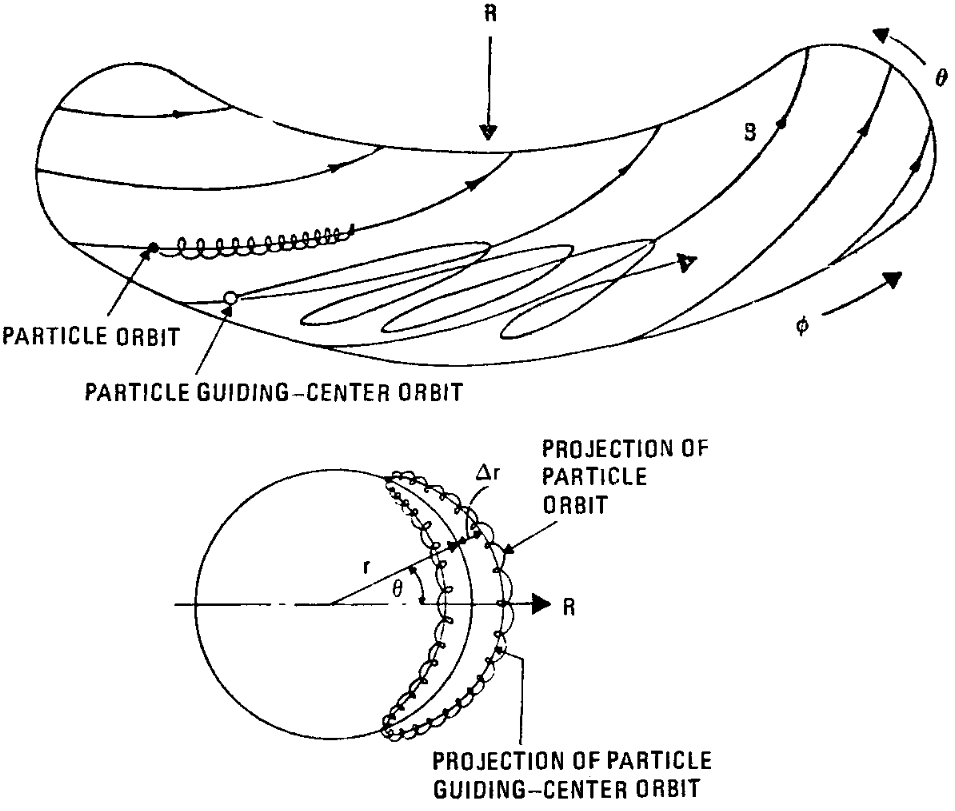
\includegraphics[width=1\linewidth]{./figures/banana.png}
        \caption{Trapped particle motion in the Tokamak exhibits a banana shape due to the toroidal magnetic field. The particle is trapped in the magnetic well and can interact with the drift wave (DW). The second figure shows a cross-section of the torus, projecting the banana orbit of the particle (From \cite{book_banana, Banana_distr_runaway}). If a wave resonates with the particle at a lower frequency than the particle's transit time, the particle can exchange energy with the wave in a quasi-adiabatic manner (see after).}
        \label{}
    \end{figure}


    \subsubsection{Drift waves}
    Electron DW instabilities that are at stake here are governed by the famous \textbf{Hasegawa-Wakatani} \cite{Hasegawa,Wakatani} equation. This equation arises due to the non-adiabatic response of the electrons, meaning that the equilibrium is not reached after each oscillation of the wave. It is derived from a simplified version of the drift kinetic equation from Vlasov theory. Therefore, let us recall the general form of the H-W equation~:
    \begin{equation}
        \begin{cases}
            \rho_s^2
            \dv{t}\nabla_\perp^2 \Phi= D_\parallel\nabla_\parallel^2(\tilde{\Phi} - \frac{T\tilde{n}}{|e|n_0}) \\
            \frac{1}{n_0}\dv{t}\tilde{n} + \frac{v_r}{n_0}\partial_r n_0 = D_\parallel\nabla_\parallel^2(\tilde{\Phi} - \frac{T\tilde{n}}{|e|n_0})
        \end{cases}\,.
    \end{equation}

    With $\rho_s$ denoting the ion sound radius, $D_\parallel$ the parallel diffusion coefficient\footnote{The parallel diffusion coefficient provides insights into the electrons-ions collision frequency: $D_\parallel = \frac{v_{the}^2}{\nu_{ei}}$}, $\Phi$ the electrostatic potential, $\tilde{n}$ the density perturbation, $v_r$ the radial velocity, $n_0$ the equilibrium density, $T$ the electronic temperature, and $e$ the electron charge.

    In the adiabatic limit \cite{Trapped_Particle_Mode}, where particles diffuse faster than the wave, we can assume a simple Boltzmann distribution of electrons with a small perturbation:
    $$\frac{\tilde{n}}{n} \approx \frac{\vert e \vert}{T} \tilde{\Phi} + \tilde{h}$$
    This leads to the \textbf{Hasegawa-Mima} \cite{Mima} equation under the assumption: $v_{thi} < \frac{w}{k_\parallel} \ll v_{the}$.

    \begin{equation}
        \begin{cases}
            \rho_s^2\dv{t}\nabla_\perp^2\tilde{\Phi} \approx \frac{1}{n_0}\left(\dv{\tilde{n}}{t} + \tilde{v_r\partial_r n_0}\right) \\
            \partial_t \frac{\vert e \vert \tilde{\Phi}}{T} + \partial_t \tilde{h} - \rho_s^2\dv{t}\nabla_\perp^2\tilde{Phi}  + v^{*}\partial_y\frac{\vert e \vert \tilde{\Phi}}{T} = 0
        \end{cases}
    \end{equation}

    With $v_* = \rho_s c_s / L_n$, where $L_n$ is the gradient scale of the equilibrium density $-\partial_r n_0 / n_0$, we obtain the following dispersion relation for the drift waves, where $w_r$ is the real frequency of the wave and $\gamma$ is the growth rate (the imaginary part of the frequency):
    $$\omega_r = \frac{w_{*}}{1 + k_\perp^2 \rho_s^2}, \quad \frac{\gamma}{w_r} = \pi \frac{w_r - w_{*}}{k_\parallel v_{e,th}}$$

    We denote $\frac{w - w_*}{k_\perp^2 v_{e,th}}$ as the non-Boltzmann factor for electron drift waves. It is important to note that this study is independent of trapped electrons; hence, the growth rate is relatively low. However, when the transit time of electrons increases (due to trapping), we find \cite{San_diego} that the non-Boltzmann factor increases, leading to a higher growth rate. This is notably because of the introduction of $w_{D,e}$, the electron curvature drift frequency. For collisionless trapped electron modes, the non-Boltzmann factor is given by:
    $$\frac{w - w_*}{w_{e,D}} e^{-R/L_n} \sqrt{\frac{R}{L_n}}$$
    which is definitively larger than the non-Boltzmann correction factor for electron drift waves.

    This leads to the following growth rate:
    $$\frac{\gamma}{w_r} = i \pi \frac{w - w_*}{w_{e,D}} e^{-R/L_n} \sqrt{\frac{R}{L_n}}$$
    explaining why \textbf{CTEM} (Collisionless Trapped Electron Modes) are much more unstable than classical electron drift waves. It also explains why the main instabilities are located in the banana region, where the coherence time of electrons is significantly longer. Similar conclusions can be drawn for the Dissipative Trapped Electron Mode \cite{Trapped_Particle_Mode}. These instabilities lead to an inverse cascade of energy (Kolmogorov), contributing to highly nonlinear interactions with mesoscale structures (zonal flows) \cite{San_diego, Krutkin_thesis, DW_transport}.
\end{multicols}
\begin{figure}[H]
    \centering
    \includegraphics[width=1\linewidth]{./figures/balloning_TEM.png}
    \caption{Cross-section view of a Tokamak with negative shear flow - On the left, we have the Fourier Ballooning mode with \( n = 6 \), characteristic of the TEM mode, presenting a characteristic tilting of the wave vector \( k_{\perp} \) and radial translational symmetry. On the right, we have a simulated TEM mode with similar shape characteristics, noting the presence of multiple modes, teared and more tilted by the zonal flow. This is explained by the nonlinear interaction between these two types of flow (reproduced from \cite{TEM_simulation, Ballooning_transform}).}
    \label{}
\end{figure}
\begin{multicols}{2}
    \subsection{Radial Transport}
    These micro-instabilities are strong candidates for explaining high radial transport. As previously discussed, resonating trapped electrons can induce significant fluctuations in the density field and magnetic pressure. Specifically, the radial particle flow does not vanish as expected; instead, there is a substantial contribution from resonant trapped electrons to the mean transport \cite{San_diego}. This radial dependency is the only density dependency retained for the following section.

    \section{Wave Propagation in Plasma}

    \subsection{Plasma as a Medium}

    To study the density profile, various diagnostic methods are available, such as Doppler Reflectometry, RCDR, and Short Pulse Reflectometry. In this study, we will focus on Short Pulse Reflectometry (\textbf{SPR}). This method involves probing the magnetized plasma with a short Gaussian pulse (less than 1 ns) of microwaves operating in the time domain at a fixed frequency and normal incidence relative to the cut-off surface. The variation in the delay of the reflected pulses is analyzed. The probing signal is sensitive to density variations, as these changes affect the cut-off position. Thus, SPR can provide deeper insights into the characteristics of turbulence.

    \subsection{Wave Equation}

    Assuming a monochromatic electromagnetic wave and using Maxwell's equations, we can derive the local complex dielectric tensor and the wave equation considered:

    \begin{equation}
        \begin{rcases}
            \laplacian E -  \vec{\nabla}\nabla \cdot E = -\frac{\omega^2}{c^2} \hat{\epsilon} E \\
            \hat{\epsilon}_{ik} = \delta _{ik} - \frac{4\pi i}{\omega} \sigma_{ik}
        \end{rcases}
    \end{equation}
    Here's the refined version of your text with LaTeX expressions retained as required:

    ---

    With $\sigma_{ik}$ representing the conductivity tensor, several assumptions have been made to establish this equation: linear Ohm's law is applicable, the plasma is considered cold \cite{cite}, and the chaotic motion of the particles, implying the neglect of kinetic effects, is disregarded. To simplify the problem further, we assume the plasma to be stationary and neglect all forms of damping. In a Cartesian coordinate system with the $z$ axis aligned with a constant magnetic field,

    $$\vec{B} = B_0 \vec{e}_z,$$

    we can derive the following dielectric tensor \cite{Thomas H. Stix}:

    $$
        \hat{\epsilon} = \begin{pmatrix}
            \epsilon & ig       & 0    \\
            -ig      & \epsilon & 0    \\
            0        & 0        & \eta
        \end{pmatrix}
    $$
    With : $\epsilon = 1 - \frac{\omega_{pe}^2}{\omega^2 - w_{ce}^2}$, $g = \frac{w_{ce}w_{pe}^2}{w(w^2 9 W_{ce}^2)} - \frac{w_{ci}w_{pi}^2}{w(w^2 9 W_{ci}^2)}$;
    $ \eta  = 1 - \frac{w_{pe}^2}{w^2} -  \frac{w_{pi}^2}{w^2}; \quad w_{pi} = \sqrt{\frac{4\pi n e^2}{m_i}}; \quad w_{ci} = \frac{eH}{m_i c}$
    Here, $\omega_{pi}$ denotes the plasma (or electron) frequency and $\omega_{ci}$ is the cyclotron frequency for the ion species. Since we are dealing with microwave frequencies, we will consider the electron component as preponderant in the subsequent study. The wave equation can thus be simplified to the following:

    \begin{equation}
        \begin{rcases}
            (S_{yz} - \epsilon)E_x - igE_y - \Pi_{xy}E_z = 0 \\
            (S_{zx} - \epsilon)E_x + igE_x - \Pi_{yz}E_z = 0 \\
            (S_{xy} - \eta)E_z -\Pi_{xz}E_x - \Pi_{yz}E_y = 0
        \end{rcases}
    \end{equation}
    Defining : $S_{ij} = N_i^2 + N_j^2; \quad \Pi_{ij} = N_iN_j ; \quad N_{i} = \frac{k_iw}{c}$
    For the \textbf{SPR} study the wave is perpendicular to the external magnetic field, hence we can simplify the system to the following :
    \begin{equation}
        \begin{rcases}
            (N_y^2 - \epsilon)E_x - igE_y = 0 \\
            (N_x^2 - \epsilon)E_y + igE_x = 0 \\
            (S_{xy} - \eta)E_z = 0
        \end{rcases}
    \end{equation}

    Which leads to two different types of solution respectively the ordinary mode ($\mathcal{O}$) and the extraordinary mode ($\mathcal{X}$).
    \setlength{\tabcolsep}{18pt}
    \renewcommand{\arraystretch}{1.5}
    \begin{center}
        \begin{tabular}{|| c  | c||}
            \hline
            $\mathcal{O}$       & $\mathcal{X}$                       \\
            \hline\hline
            $S_{xy} - \eta = 0$ & $(N_y^2 - \epsilon)E_x - igE_y = 0$ \\
            $E_y = 0$           & $(N_x^2 - \epsilon)E_y + igE_x = 0$ \\
            $E_x = 0$           & $E_z = 0$                           \\
            \hline
        \end{tabular}
    \end{center}

    The $\mathcal{O}$ mode corresponds to the mode with the electric field parallel to the external magnetic field. Therefore, the propagation of this mode depends solely on the density profile and is independent of the magnetic field. In contrast, the $\mathcal{X}$ mode has the electric field perpendicular to the external magnetic field. Consequently, the propagation of the $\mathcal{X}$ mode depends on both the magnetic field and the density profile.

    The dispersion relation of the wave can be derived locally from the wave equation. We obtain:
    \begin{equation}
        k^2 = \frac{w^2}{c^2} \eta \approx \frac{w^2}{c^2}\left(1 - \frac{n}{n_c}\right); \quad n_c = \frac{m_ew}{4 \pi e^2}
        \label{eq:Dispersion_relation}
    \end{equation}

    Here we can see that the wave number vanishes at \( n = n_c \), which is the cut-off layer where the wave is reflected. The \( k \)-spectrum of the $\mathcal{X}$ mode is much more complicated and includes plasma resonances where thermal effects must be taken into account. For this study, we will limit ourselves to the $\mathcal{O}$ mode.

    From solving the Helmholtz equation (local dependency of the wave number):

    $$
        \pdv[2]{E_z}{x} + k(x)E_z = 0
    $$

    and applying the \textbf{WKB} approximation (slow variation of the plasma parameters), i.e., assuming a solution of the form \( E_z = A(x) \exp(i\Phi(x)) \), with \( A \) varying slowly and \( \Phi \) varying quickly, we can derive the following expression for the electric field:

    $$
        E_z(x) = \frac{E_z}{\sqrt{\frac{c}{\omega}k(x)}}\exp\left(i\int_0^x k(x')dx'\right)
    $$

    The WKB approximation will be used in the one-dimensional approach (see Chapter 2) and in the \textbf{CUWA} code for computing ray tracing in order to adjust the size of computation Yee cells \cite{CUWA} and the computation domain.

    \section{CUWA Code Overview}

    The CUWA code is a \textbf{GPU}-based computation scheme with a Python-CUDA framework, using a finite difference scheme for spatial dependency applied to the three different fields: \( E \), \( B \), and \( J \), along with the well-known leap-frog time stepping. It is used to simulate the propagation of electromagnetic waves inside a \textit{"cold plasma"}. The spatial finite difference scheme is based on the FDTD Yee's method \cite{Yee}, with slight modifications. It solves the discrete version of Maxwell's equations with a cold plasma current response \( \textbf{J} \):

    \begin{equation}
        \begin{cases}
            \pdv{t}\textbf{B}  = - \nabla \times \textbf{E}                                                 & \text{} \\
            \pdv{t}\textbf{E} = c^{2}\nabla \times \textbf{B} - \frac{\textbf{J} }{\epsilon_0 }             & \text{} \\
            \dv{t} \textbf{J} \nu \textbf{J} = \epsilon_0 w_p^2 \textbf{E} - \textbf{J} \times \textbf{w}_c & \text{} \\
        \end{cases}
        \label{eq:Maxwell}
    \end{equation}
    with $w_p$ the electron plasma frequency, $\nu$ the electron collision frequency, and $w_c$ the electron cyclotron frequency. To limit the computational cost, the computation domain is amended with a convolutional perfectly matched layer (\textbf{PML}) to ensure that any reflected signals are minimal (well-used in open boundary systems). It can be viewed as a sponge layer for electromagnetic waves.
\end{multicols}
\noindent
\rule{\linewidth}{0.4pt}

\begin{figure}[H]
    \centering
    \hspace*{-.17cm}\includegraphics[width=1.02\linewidth]{./figures/field_SPR.pdf}
    \caption{\textbf{SPR} setup using the \emph{O. Krutkin and A. Combette \textbf{LEONARDO} simulations from the \textbf{CUWA} code}. The probing wave is sent to the plasma, and the reflected wave from the cut-off is measured. The delay between the two waves provides a measure of the plasma density profile, in addition to the pulse shape altered by the turbulence (eq). Here we plot the contours of the density profile, with cold density perturbations (black contour lines on the left plot). The probing wave is reflected by the cut-off layer (initial probing wave on the left and after a $\Delta t \approx 10 \, \text{ns}$ we get the reflected scattered wave on the right). The third plot on the right shows the density profile with its perturbations (filled). A linear density profile
        \[ n(x,y) = \frac{x}{L} \left(n_c + \delta n(x,y)\right) \]\
        has been chosen according to (cite). Note that this linear correction made on the amplitude of the turbulence fields follows from the non-adiabatic perturbations \cite{San_diego} and numerical instability, and is more relevant than a simple constant amplitude turbulence field. The curvature of the grid has been set to \( R = 0.25 \, \text{m} \) to mimic the TCV geometry.}
    \label{}
\end{figure}

\begin{multicols}{2}

    \section{Linear Regime Study}
    The goal of this study is to find a way to link the plasma density perturbations to the reflected pulse characteristics. First, we will study a simple 1-dimensional model proposed by (\emph{Oleg Krutkin}) applied in a given range of turbulence amplitudes and sizes, and then we will extend this study to a more general 2D model using the \textbf{CUWA} code.

    Assuming a simple plasma density profile $n(x)$, we can study the wave propagation in the plasma. The goal of this approach is to find a way to link the plasma density perturbations to the reflected pulse delay. To retrieve information about the pulse delay, we will use a statistical approach to account for the randomness introduced by perturbations.

    The delay of the probing wave is given by the following formula:
    $$\tau_c = 2 \int_0^L \frac{dx}{v_g},$$
    where $v_g$ is the group velocity of the wave, and $L$ is the position of the cut-off.

    From the simple assumption $\langle \delta n \rangle = 0$ for an Ordinary mode, the $v_g$ expression obtained can be used to expand the integral to:
    $$\frac{2}{c} \int_0^L \frac{dx}{\sqrt{1 - \frac{x}{L} - \frac{\delta n }{n_c}}}.$$
    The main contribution of this integral comes from the vicinity of the cut-off layer, where the group velocity is the smallest.

    We can discuss the relevance of this expansion as the main contribution of the integral comes from the cut-off region where the WKB approximation cannot be applied.

    \subsection{Perturbed Density Profile}
    \subsubsection{General Perturbation Profile}
    First, let's consider a Gaussian perturbation density profile (we will see later that the spectrum of the wave vector is not Gaussian but a non-trivial power spectrum due to the two types of energy cascades). From this, the considered integral can be written as:
    $$\tau_d = \frac{2}{c} \int_0^L \frac{dx}{\sqrt{1 - \frac{x}{L} - \frac{\delta n_0 \exp\left(-\frac{(x - L)^2}{8l_{cx}^2}\right)}{n_c}}}.$$
    With $l_{cx}$ as the correlation length of the turbulence field and $\delta n_0$ as the amplitude of the turbulence field. This integral is not trivial to solve analytically, which is necessary to exhibit the possible statistical features of the delay. Therefore, we suggest developing a first-order perturbation profile that leads to step-like perturbations.

    \subsubsection{Step-like Perturbation}
    \paragraph*{Model}
    With a step-size perturbation characterized by $l_{cx}$ length, we can derive an analytical expression for the integral for different density profiles. To simplify, we assume the perturbation is small enough such that the WKB approximation can be applied. This is valid for the linear regime, where the perturbation is small enough such that the cut-off layer is not significantly perturbed (i.e., $\delta_x \ll l_{cx}$). In the case of a large perturbation, another step perturbation localized far from the cut-off layer can be used to obtain similar results, though this breaks the main assumption of this approach (see fig.1).

    It is relatively straightforward to obtain the following expression for the delay [cite Krutkin]:
    $$\tau_d = \frac{4L}{c} - \frac{2L}{c} \sqrt{\frac{L}{l_{cx}}} \frac{\delta n}{n_c}.$$

    The statistical approach is to consider the perturbation as a random variable and compute the statistical properties of the delay of the probing wave. This approach is relevant for the linear regime, where the perturbation is small enough such that the cut-off layer is not significantly perturbed (i.e., $\delta_x \ll l_{cx}$). For example, we can compute the standard deviation of the delay depending on the standard deviation of perturbations. This yields:
    $$\sigma_{\tau_d} \approx \frac{2L}{c} \sqrt{\frac{L}{l_{cx}}} \frac{\sigma_{\delta n}}{n_c}.$$

    To test this assumption, we can compare the analytical expression with the numerical integration of the wave equation for numerous Gaussian perturbations with characteristic length $l_{cx}$ and various amplitudes $\delta n$, as depicted in Figure \ref{fig:std_delay}.
\end{multicols}
\noindent
\rule{\linewidth}{0.4pt}

\begin{figure}[H]
    \centering
    \hspace*{-0.8cm}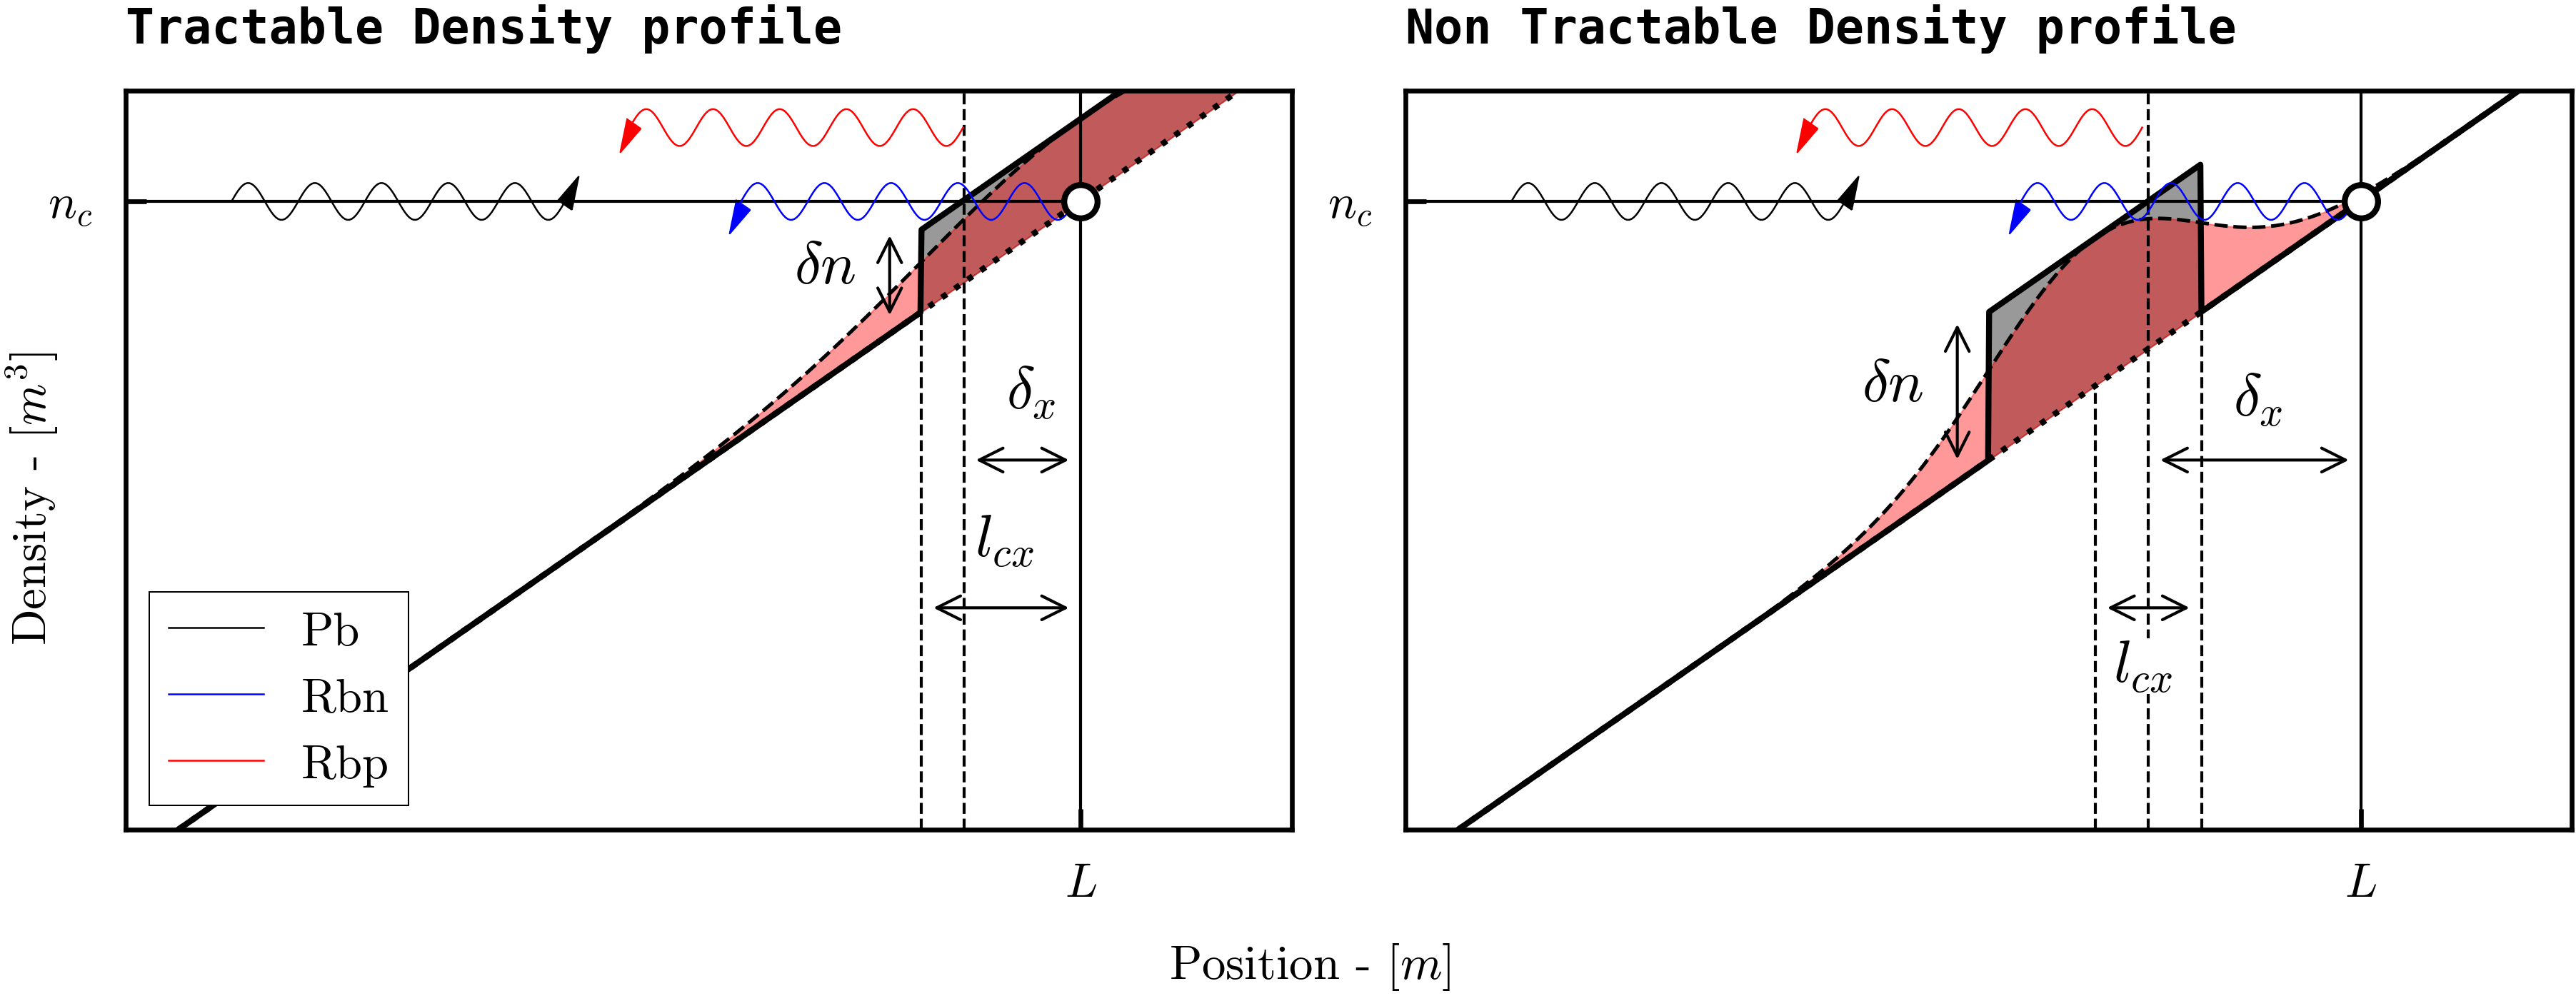
\includegraphics[width = 1.03\linewidth]{./figures/density_profile.png}
    \caption{Here we plot the density profile of the plasma for different perturbation amplitudes: in grey, the step-like model perturbation and in coral, the Gaussian one. For large value density perturbations, the model leads to a contradiction with its assumption \(\delta x < l_{cx}\) or \(\delta n < n_c \frac{l_{cx}}{L}\), indicated by a small cut-off layer shift. The blue Pb wave is the probing wave, the red Rbp wave is the reflected one, and the blue Rbn wave is the normal reflected wave in the absence of perturbation.}
    \label{Density_profile}
\end{figure}

\begin{multicols}{2}
    One sample of density fluctuation is produced using the following formula, to match a supposed gaussian spectra of instabilities :
    $$\delta n(k_x) = \delta n_0 \exp\left(-\frac{(kl_{cx})^2}{8} + i\Phi(k)\right)$$
    with $\Phi(k)$ a random phase, k the radial wavenumber of the density perturbation and $\delta n_0$ the amplitude of the perturbation, this amplitude can be taken constant or dependant of the radial position according to the kind of profile we use. Then we inverse fourrier transform this density perturbation to get the density profile in the real space. Finally, for each sample, the delay is then numerically integrated from the formula [cite delay], using simple trapezoidal integration.
    \paragraph*{Results}
    The results are shown in Figure \ref{fig:std_delay}. The simulated deviation of delay which serves as reference (black crosses) was computed from 10,000 samples to ensure statistical stability, using a 50 GHz probing wave and a $2L$ integration domain. This setup allows us to account for negative perturbations near the cut-off, as multiple perturbations near the standard cut-off might strongly shift it. The plain black line represents the first-order approximation of the formula [eq], while the dashed line denotes the third-order approximation of the second formula.

    For reproducibility, the parameters of the 1D simulation used to build the considered datasets are given below:
    \setlength{\tabcolsep}{.038\linewidth}
    \renewcommand{\arraystretch}{1.5}
    \begin{center}
        \begin{tabular}{ccccc}
            \toprule
            \multicolumn{5}{c}{Parameters range}                       \\
            \cmidrule{1 -5}
            $\delta n_0$   & $l_{cx}$ -[cm] & L -[cm]  & $N_x$ & n     \\
            \midrule
            $[1e^{-3}, 1]$ & $[0.1,1]$      & $[7,20]$ & 5000  & 10000 \\
            \bottomrule
        \end{tabular}
    \end{center}


    The second-order analytical formula exhibits a characteristic drop-off after reaching a critical amplitude value, similar to the simulated delay. This suggests that expanding further the $\sigma_{\tau_d}$ could improve handling of the non-linear domain. However, discrepancies are observed for large perturbations in the non-linear regime, though the analytical expression provides a good approximation for small perturbations, except for very tiny ones [cite].

    Note that the critical value can be defined in two ways \cite{SPR_Krutkin, PUT} and sets the threshold for what could later be considered the \textbf{non-linear} regime. Indeed we can consider the critical amplitude of turbulence as the densoty threshold where the 1D model is not applicable i.e when : $$\delta n \geq n_c \frac{L_{cx}}{L} = \delta n_{c 1}$$ This first approach does not care information about the multiple scattering of the pulse, which leads to extinction of the probing line and saturation of the scattered signal power (CITE). This random non-linear scattering effect has already been studied for RCDR and DR theory \cite{critical2}, and leads to thefollowing formula :

    $$ \frac{\delta n}{n_c} \gg  \frac{c}{w\sqrt{l_{cx}L\ln{\frac{L}{lcx}}}} = n_{c2}$$

    In our case, the second critical value $n_{c 2}$ is below $n_{c 1}$, and we will see that it will influence the future parametrization of our model.

    A correction factor dependent on $l_{cx}$ should be introduced to achieve better agreement with the numerical integration. This factor has not been studied yet but highlights the limitations of the current step-driven 1D model. \footnote{The integration of the Gaussian integral was also tackled, with a second-order bell-approximation, leading to logarithmic dependencies over the plasma parameters. However, the formula was too complex to exhibit the statistical properties of the delay, as referred to in the appendix.} As highlighted before, the non-linear regime is strongly related to scattering effects, which are not considered in this approach. Additionally, density corrugations can reach up to 100\% of the density value near the cut-off \cite{Krutkin_thesis,San_diego}, especially since the adiabatic and non-adiabatic components of the electron response have the same potential dependency \cite{San_diego}. Therefore, the non-linear regime is significant, and a sufficiently precise model is necessary to evaluate turbulence amplitudes in the \textbf{NL} regime.

    \begin{figure}[H]
        \centering
        \hspace*{-0.2cm}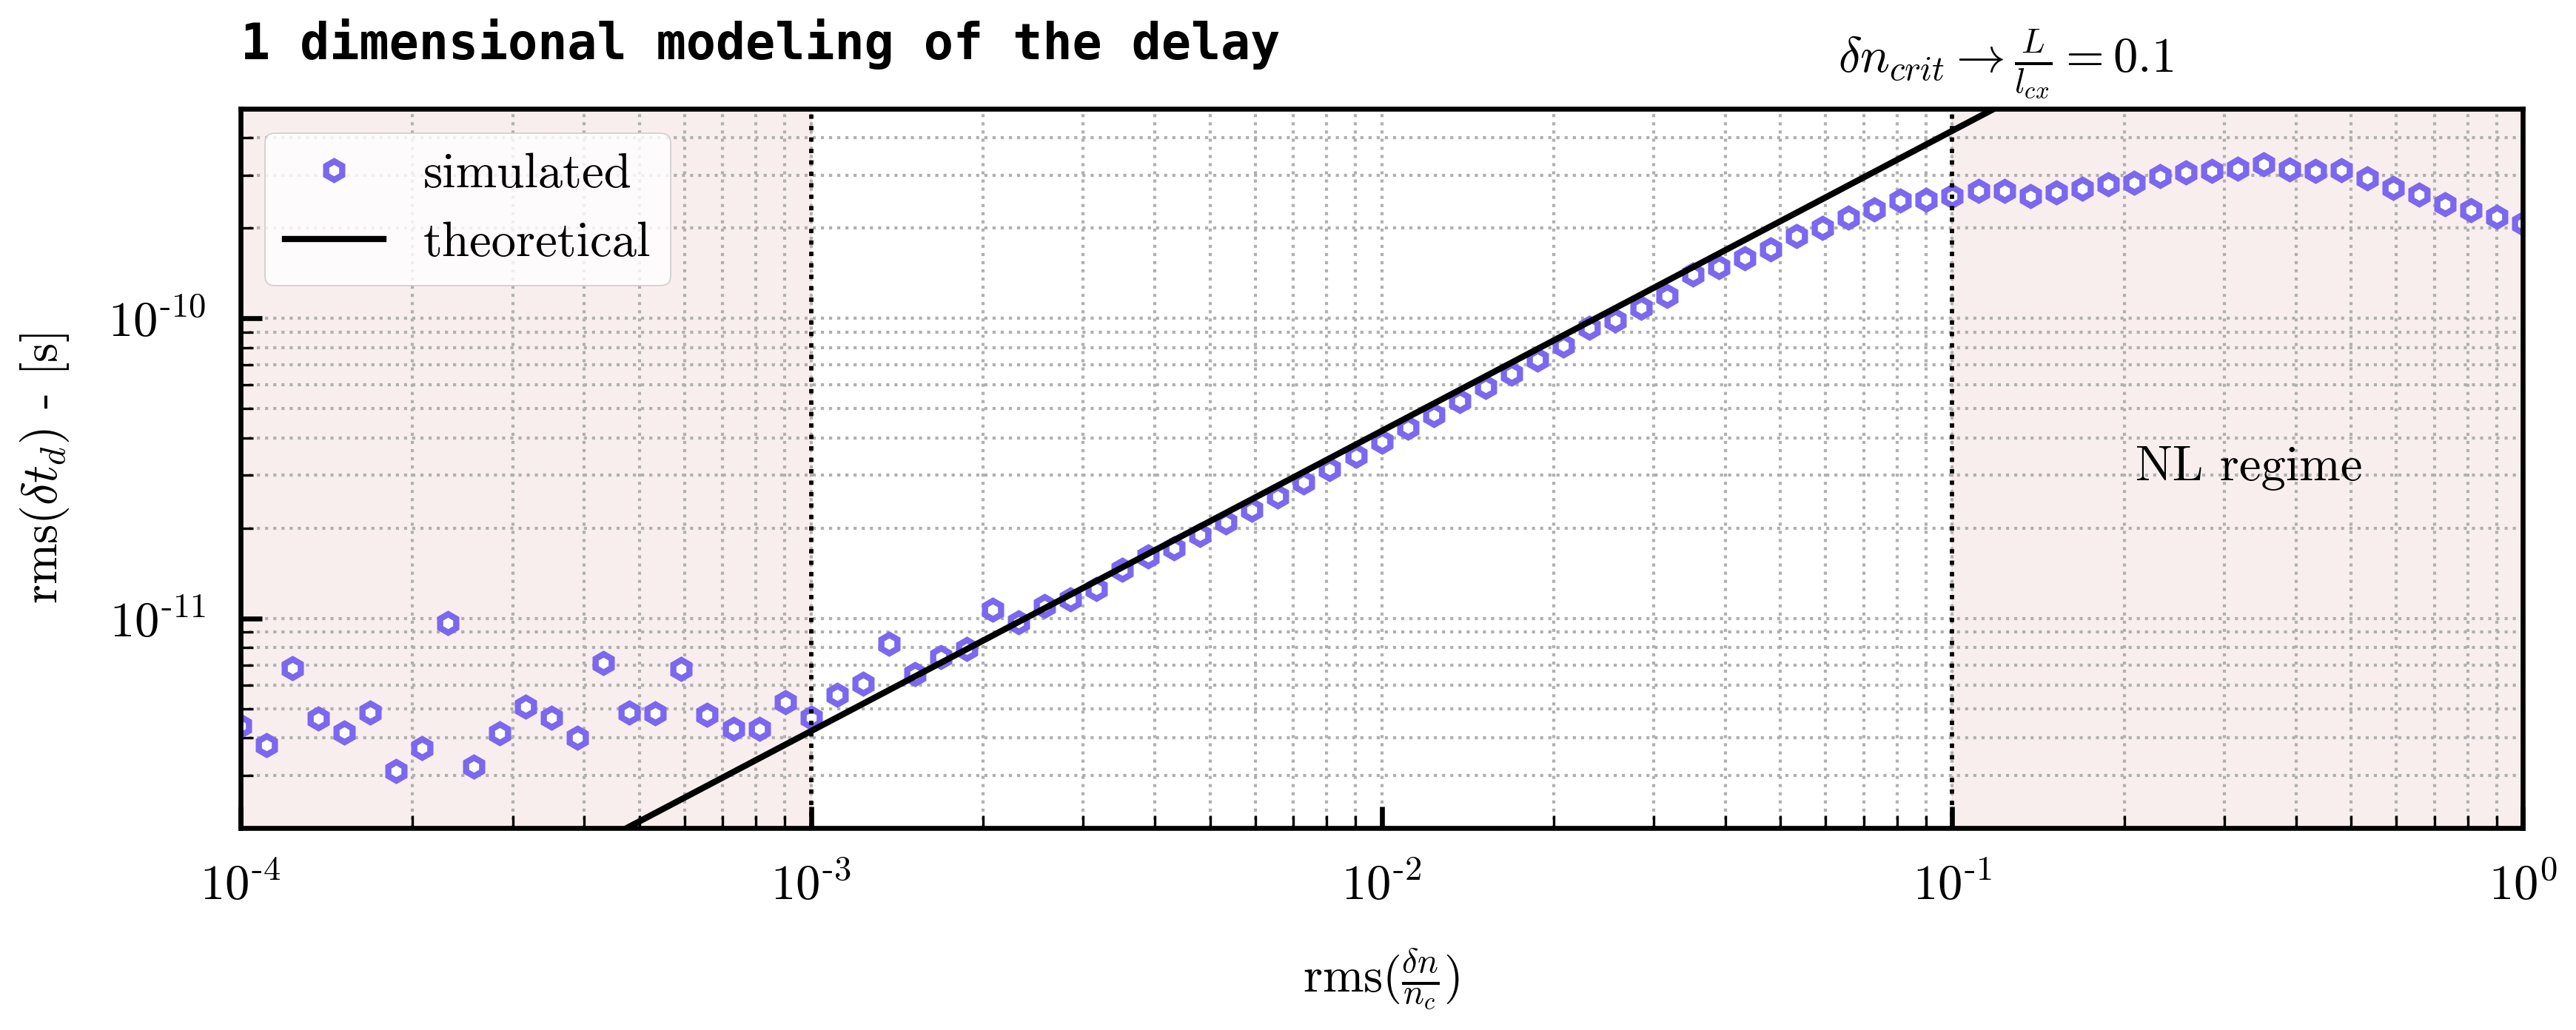
\includegraphics[width=1.2\linewidth]{./figures/1d.pdf}
        \caption{1-dimensional predicted amplitude of the analytical 1st and 2nd order step-driven model, compared to the simulated 1-dimensional delay (see eq: \ref{eq:Dispersion_relation}). A constant \(\delta n_0\) has been used for the density profile.}
        \label{fig:std_delay}
    \end{figure}

    Hence, the first issue that arises is finding a good parametrization of the model, i.e., identifying the best statistical metrics to predict the amplitude of the turbulence. This study will use several profiles of density perturbations amplitudes $\delta n_0$ to determine if the model we build is sufficiently robust to adapt.

    \chapter{1-Dimensional Model}

    The first model we developed relies on the 1-dimensional integration of the delay. For this simple model, we can only use the pulse delay's statistical properties. Several options were tested, including studying the quantile distribution of the delay, its histogram, and various statistical properties. The study involves a simple multi-dimensional regression problem where we attempt to estimate the amplitude of the perturbation and the non-perturbed delay of the probing wave (i.e., without the turbulence fields) for several density profiles. To address this, we used a stacked regressor combined with a multi-output regressor.

    \section{Reliable Metrics}

    To train our machine learning model, we need clear data with the best input possible. First, let's examine the characteristics of the delay. To get a general overview of the influence of the turbulence amplitude $\delta n_0$ on the delay characteristics, we study the distribution of the delay as a function of the amplitude. This is illustrated in the following plot.

    \begin{figure}[H]
        \centering
        \includegraphics[width=1\linewidth]{figures/delay_overview.pdf}
        \caption{Violin plots of the delay distribution over \(\delta n_0\). For a straightforward initial approach, we selected a simple linear profile with \(\delta n_0\) independent of the radial position. The left side of each violin represents the 2D distribution of the delay for comparison.}
        \label{fig:Violins_delay}
    \end{figure}
    The first observation is that the delay distribution is significantly affected by the amplitude increase. As the amplitude grows, the mean delay decreases (which is expected, see \ref{fig:Density_profile}), and the standard deviation of the delay increases before decreasing when the non-linear regime is reached. Additionally, the distribution becomes more skewed until reaching the non-linear regime charcterized here by the first crtical value $n_{c1}$ , this broadening suggests that studying the moments of the delay distribution could also be a useful method for predicting the amplitude level.

    The two simulation sets exhibit similar behavior, but discrepancies arise at high amplitudes. Specifically, the 1D simulation set shows more erratic distributions compared to the 2D simulation set, raising questions about the convergence of the 1D integration (see: \ref{eq:Dispersion_relation}). It is noteworthy that the critical density identified in this plot is the first critical density (CITE), which is crucial for constructing a qualitative dataset. Despite these concerns, the delay study appears to provide a reasonable estimate for amplitude levels in both simulation sets, even without analyzing pulse shapes as done in the 2D model.

    Hence, the next step is to evaluate whether the delay study can effectively estimate amplitude levels in both 1D and 2D scenarios.

    \section{Machine Learning Model}

    The machine learning model will be trained to predict the amplitude $\delta n_0$ and the default delay without amplitude $\tau_0$, using a one-dimensional training set and tested on both one-dimensional and two-dimensional test sets.

    \subsection{Structure}

    The regression model we used is a stacked multi-output regressor.

    \begin{figure}[H]
        \def\svgwidth{\linewidth}
        \centering
        \input{./figures/stacked_regressor.pdf_tex}
        \caption{Stacked Regressor structure with a global regressor chain. The internal structures of the multiple regressors are not detailed for simplicity, but each one is a complex model with specific advantages and limitations. Each model was tested on several datasets, and their combination is key to the performance of our predictions, especially in extreme cases with high or low turbulence amplitudes.}
    \end{figure}


    The following table describes the hyperparameters used for the stacked model.

    \begin{table}[H]
        \centering
        \begin{tabularx}{1\linewidth} {
                || >{\centering\arraybackslash}X
                | >{\centering\arraybackslash}X  ||}
            \hline
            \textbf{Model} & \textbf{Hyperparameters}                                                                                    \\
            \hline\hline
            \texttt{KNN}   & \begin{tabular}[c]{@{}c@{}}\texttt{n\_neighbors} : 20 \\ \end{tabular}                                      \\
            \hline
            \texttt{RF}    & \begin{tabular}[c]{@{}c@{}}\texttt{n\_estimators} : 300\\ \texttt{max\_depth} : 40\end{tabular}             \\
            \hline

            \texttt{GB}    & \begin{tabular}[c]{@{}c@{}}\texttt{n\_estimators} : 200\\ \texttt{lr} : 0.005\end{tabular}                  \\
            \hline

            \texttt{LGBM}  & \begin{tabular}[c]{@{}c@{}}\texttt{n\_estimators} : 200\\ \texttt{lr} : 0.005\end{tabular}                  \\
            \hline

            \texttt{XGB}   & \begin{tabular}[c]{@{}c@{}}\texttt{n\_estimators} : 200\\ \texttt{lr} : 0.005\end{tabular}                  \\
            \hline

            \texttt{SVR}   & \begin{tabular}[c]{@{}c@{}}\texttt{kernel} : 'rbf'\\ \texttt{C} : 1 \\ \texttt{epsilon} : 0.01\end{tabular} \\
            \hline
        \end{tabularx}
        \caption{Main Hyperparameters used for the stacked model, the error used is not detailed as long as the performance tweaks}
        \label{Hyperparameters}
    \end{table}

    Our model combines the following models: K-neighbors (\texttt{KNN}), Random-forest (\texttt{RF}), three different Gradient-Boosting (\texttt{GB}, \texttt{LGBM}, \texttt{XGB}), and Support Vector Regressor (\texttt{SVR}). It is designed to be as general and versatile as possible. The six models are trained in parallel on the same training datasets and then combined in series with a decision regression model, which, in our case, is a final \texttt{RF} layer trained on the outputs of the previous layers. Normally, Gradient-Boosting models cannot handle multi-output regression, which is why we used a multi-output \href{https://scikit-learn.org/stable/modules/generated/sklearn.multioutput.RegressorChain.html}{\texttt{RegressorChain}}. This model trains to predict the first entry and then predict the second given the first prediction. This allows for incorporating a dependency between the different outputs, which should not be the case here, so a simple \texttt{MultiOutputRegressor} should suffice. Note that the score of the final model cannot be lower than the score of the best individual model.



    \section{Input Data}


    \section{Datasets building}

    For the 1D-based trained model, we can only use the delay distribution as input variables. We tried several moments of the distribution as input (mean, variance, skewness, etc.), combined with the discretized delay distribution. We tested two types of discretization: the binned distribution (i.e the histogram of delay) and the quantile distribution. However, we obtained better results with the quantile study of the distribution, coupled with the moments as inputs. This approach allows the model to have a direct connection between the output $\tau_0$ and the quantilized distribution. We first noticed an increasing of accuracy of models with the increasing of the number of quantile until 30 quantiles, when the efficiency of the model begins to saturate and decrease. This is why we used 30 quantiles to discretize the distribution in both cases. The 1D simulation set was then processed, split into a training and a testing set (80/20 ratio), and finally standardized. The amplitude parameter was used with its logarithmic value because it was found to be more efficient. Thus, we arrived at a final input shape of 33 features and approximately 3000 samples, including the $L$ and $l_{cx}$ parameters in the input data. For the 1D simulation, we introduced a random shift in the delay distribution for each sample. If we did not do this, the model would learn the $\tau_0$ value from the highly correlated parameter $L$ (originally, $L$ is linear with $\tau_0$), which might not be the case in experimental data, where $L$ can represent the gradient scale at the cut-off \cite{Krutkin_thesis}. For this study, we used several density profiles to see if they impact the learning process of the model. For the 1D simulations, the dependency over $y$ is dropped.

    For the linear background profile, the global density profile will be:
    $$n(x,y) = n_c \frac{x}{L} + \delta n_0(x) \delta n(x,y).$$
    Here, $\delta n$ is the normalized 2D Gaussian turbulence profile.

    For the quadratic background profile, $L$ stands for the gradient scale at the cut-off, and $\delta n_0$ is the turbulence amplitude profile. We used the following formula to get a gradient value of 1 at $L$:
    $$n(x,y) = n_c \left[1.25 - \frac{(1.5L_0 - x)^2}{L_0^2} \right] + \delta n_0(x) \delta n(x,y).$$
    The negative values of the profiles are then shifted to zeros to prevent unphysical events, which has the effect of creating a larger vacuum layer in the simulations, and then a shift of the delay distribution. This explains partially why our model need to decorlate the delay from the $L$ parameter (see section PUT).

    The dependency of $\delta n_0$ will take several forms, from constant to linear, quadratic, or exponentially weighted \cite{SPR_Krutkin}. This scaling of the turbulence is done to mimic the true turbulence profile (REF) and to avoid the unnatural predominance of turbulence while working with small amplitudes. This exploration of the density profile is motivated by the fact that at the edge of the plasma, the relative amplitude of the turbulence profile is higher than in the core of the plasma.

    The parameters of the 1D simulation are given below.
    \setlength{\tabcolsep}{.03\linewidth}
    \renewcommand{\arraystretch}{1.4}
    \begin{center}
        \begin{table}[H]
            \begin{tabular}{ccccc}
                \toprule
                \multicolumn{5}{c}{Parameters range}                       \\
                \cmidrule{1 -5}
                $\delta n_0$   & $l_{cx}$ -[cm] & L -[cm]  & $N_x$ & n     \\
                \midrule
                $[1e^{-3}, 1]$ & $[0.1,1]$      & $[7,20]$ & 5000  & 10000 \\
                \bottomrule
            \end{tabular}
            \caption{Range of parameters used for the 1D simulations. A grid was employed to ensure homogeneous learning across the entire parameter space, potentially leading to stepped regression with constant values between points in the space.}
            \label{1d_params}
        \end{table}
    \end{center}
    \section{Results}
    A good way to evaluate the model is to study the residuals for each parameter value in the testing set. This approach provides a quick overview of the model's performance and the impact of parameter values on the model's accuracy.
    \begin{figure}[H]
        \includegraphics[width=0.98\linewidth]{./figures/polar_param_1d.pdf}
        \caption{Plot of the amplitude residuals of the model for the 1D testing set in Non linear regime, the residuals are meaned given a value of the studied simulation's parameter. The filled curved stands for the amplitude residuals exponentially rescaled to the real amplitude value, The red line in the center of the plot is the $\tau_0$ mean residuals, far bellow the mean amplitude residuals. The second smaller polar shows the comparison of the residuals for several daasetets : the plot of the mean amplitude residuals for the 2D datasets (black dashed curve), the amplitude residuals for the 1D datasets (blue curve in the center), and the plots of the residuals for the 2D datasets shifted to the 1D delay distribution (green curve). The black points around the circle show the values taken by the parameter, deduced by the range given in the table PUT}
        \label{fig:polar_1d}
    \end{figure}
    From this, we reach a final score of 0.94 without the moments and 0.96 with the moments on the 1D test datasets. However, with the 2D datasets, the results are catastrophic. The model generally predicts an amplitude level one order of magnitude below or above the actual value.

    The figure \ref{fig:polar_1d} reveals quite good results for the 1D model prediction on the 1D testing simulation datasets. The predicted values are generally of the same order of magnitude as the real ones, and the residuals are well-distributed across all simulation parameters, which is encouraging. However, when generalizing the model to higher dimensions, specifically 2D simulations, we encounter very poor results with a mean amplitude residual value of 10 for any simulation parameters. This discrepancy can be attributed to the fact that 1D simulations do not account for multiple scattering effects in the nonlinear regime (see \ref{eq:Dispersion_relation}). Notably, in the nonlinear regime, the 1D testing simulation datasets show that the model performs significantly better than the analytical approach. Nevertheless, one can question whether the delay distribution between 2D and 1D cases is similar. For the same 1D parameters, there is a shift in the mean value of the delay between 2D and 1D simulations. This shift is due to the added void layer around the computation domain in the 2D simulations \cite{SPR_Krutkin} and the fact that the pulse is not launched at $t=0$. If we adjust the 2D simulation delay datasets to match the 1D simulation delay (though this adjustment is debatable), we achieve quite a good score even in the nonlinear regime (this observation was made with a flat 2D geometry and does not account for crucial 2D simulation parameters such as the probing angle or the curved profile). The residuals are approximately twice the amplitude value, which is relatively good considering the logarithmic scale of the amplitude during the training process.

    However, it is worth investigating whether studying the pulse shape with different characteristics could lead to better results. Such an approach would allow us to account for multiple scattering effects and the dispersive effects of the plasma. This will be the subject of the next chapter.

    \chapter{2-Dimensional Model}

    Considering a 2-dimensional model allows us to take into account several interesting effects that play a significant role in the \textbf{SPR} diagnostic. Indeed, the 1D model restricted the study to delay distribution. With the CUWA 2D simulations, in addition to the delay, we can study the pulse shape and its statistical properties. Furthermore, this additional dimension supports the curvature $\frac{1}{R}$ study implied by the tokamak geometry. We can also adjust the probing wave incidence angle $\theta$ and this 2 dimensional approach allows taking into account multi-scattering effect in our model. We will study the impact of these new model parameters on performance and determine if adding more complexity to the model can lead to better results with the 2D simulation datasets.

    \section{Pulse Shape Study}

    The goal of the pulse shape study is to find the best metrics that carry the most information regarding pulse shape characteristics. We will study the evolution of the pulse amplitude over the increasing of the turbulence ampliude, the number and the assymetry of scattered pulses, and their impacts on the final recording (broadening of the mean pulse), etc. This will help in building a more accurate model without adding excessive dimensions to the input layer.

    \subsection{Relative Study of Pulse Shape}

    For this part of the study, we will limit ourselves to a simple slab geometry with normal probing, without considering any curvature or incident angle. The pulse shape can provide information about the plasma density profile, as it can be modified by perturbations due to multiple scattering effects and dispersive effects [see \ref{eq:Dispersion_relation}].

    The dependence of the pulse shape on the background density profile will also be studied with linear, quadratic, and linearly modified perturbation profiles. We expect to observe a much larger and more randomly dependent pulse at high turbulence amplitudes due to multiple scattering. The reflected pulse will be a superposition of all scattered pulses, characterized by a growing tail in both delay and width.

    \begin{figure}[H]
        \centering
        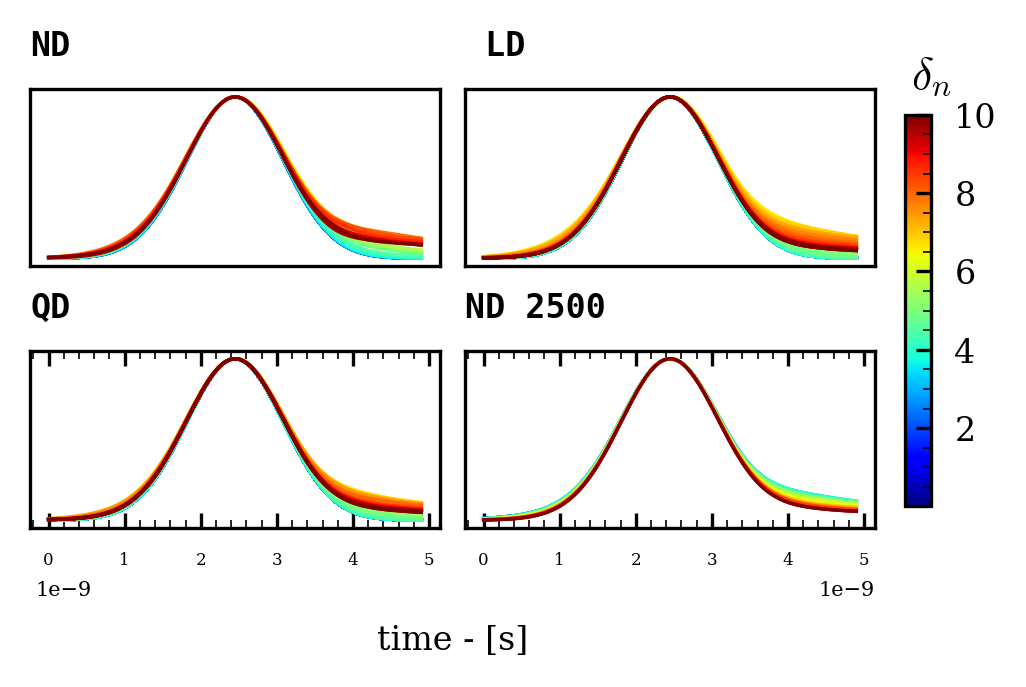
\includegraphics[width=1\linewidth]{./figures/pulse_shape.png}
        \caption{Normalized mean of reflected pulse signal for several density profiles. \textbf{ND} represents a linear density profile with a linear dependency of $\delta n_0$ over $x$, \textbf{LD} is a simple linear density profile with a constant turbulence amplitude, \textbf{QD} is the quadratic density profile, and \textbf{ND 2500} is a 2500-sample simulation (the amplitude range is not respected for this one due to computation cost).}

        \label{fig:barrier}
    \end{figure}
    For all density profiles, the pulse shape becomes broader for larger perturbations, and the delay increases.

    This broadening is due to multiple scattering and dispersive effects. From this overview of the normalized mean pulse shape, it is evident that an interesting metric for our model should measure how much the mean pulse is skewed. This can be characterized by studying the mean skewness of the pulse shape. Another interesting parameter to highlight is the hysteresis of the normalized mean pulse (i.e., the ratio of the right area to the left area of the pulse).
    \begin{figure}[H]
        \centering
        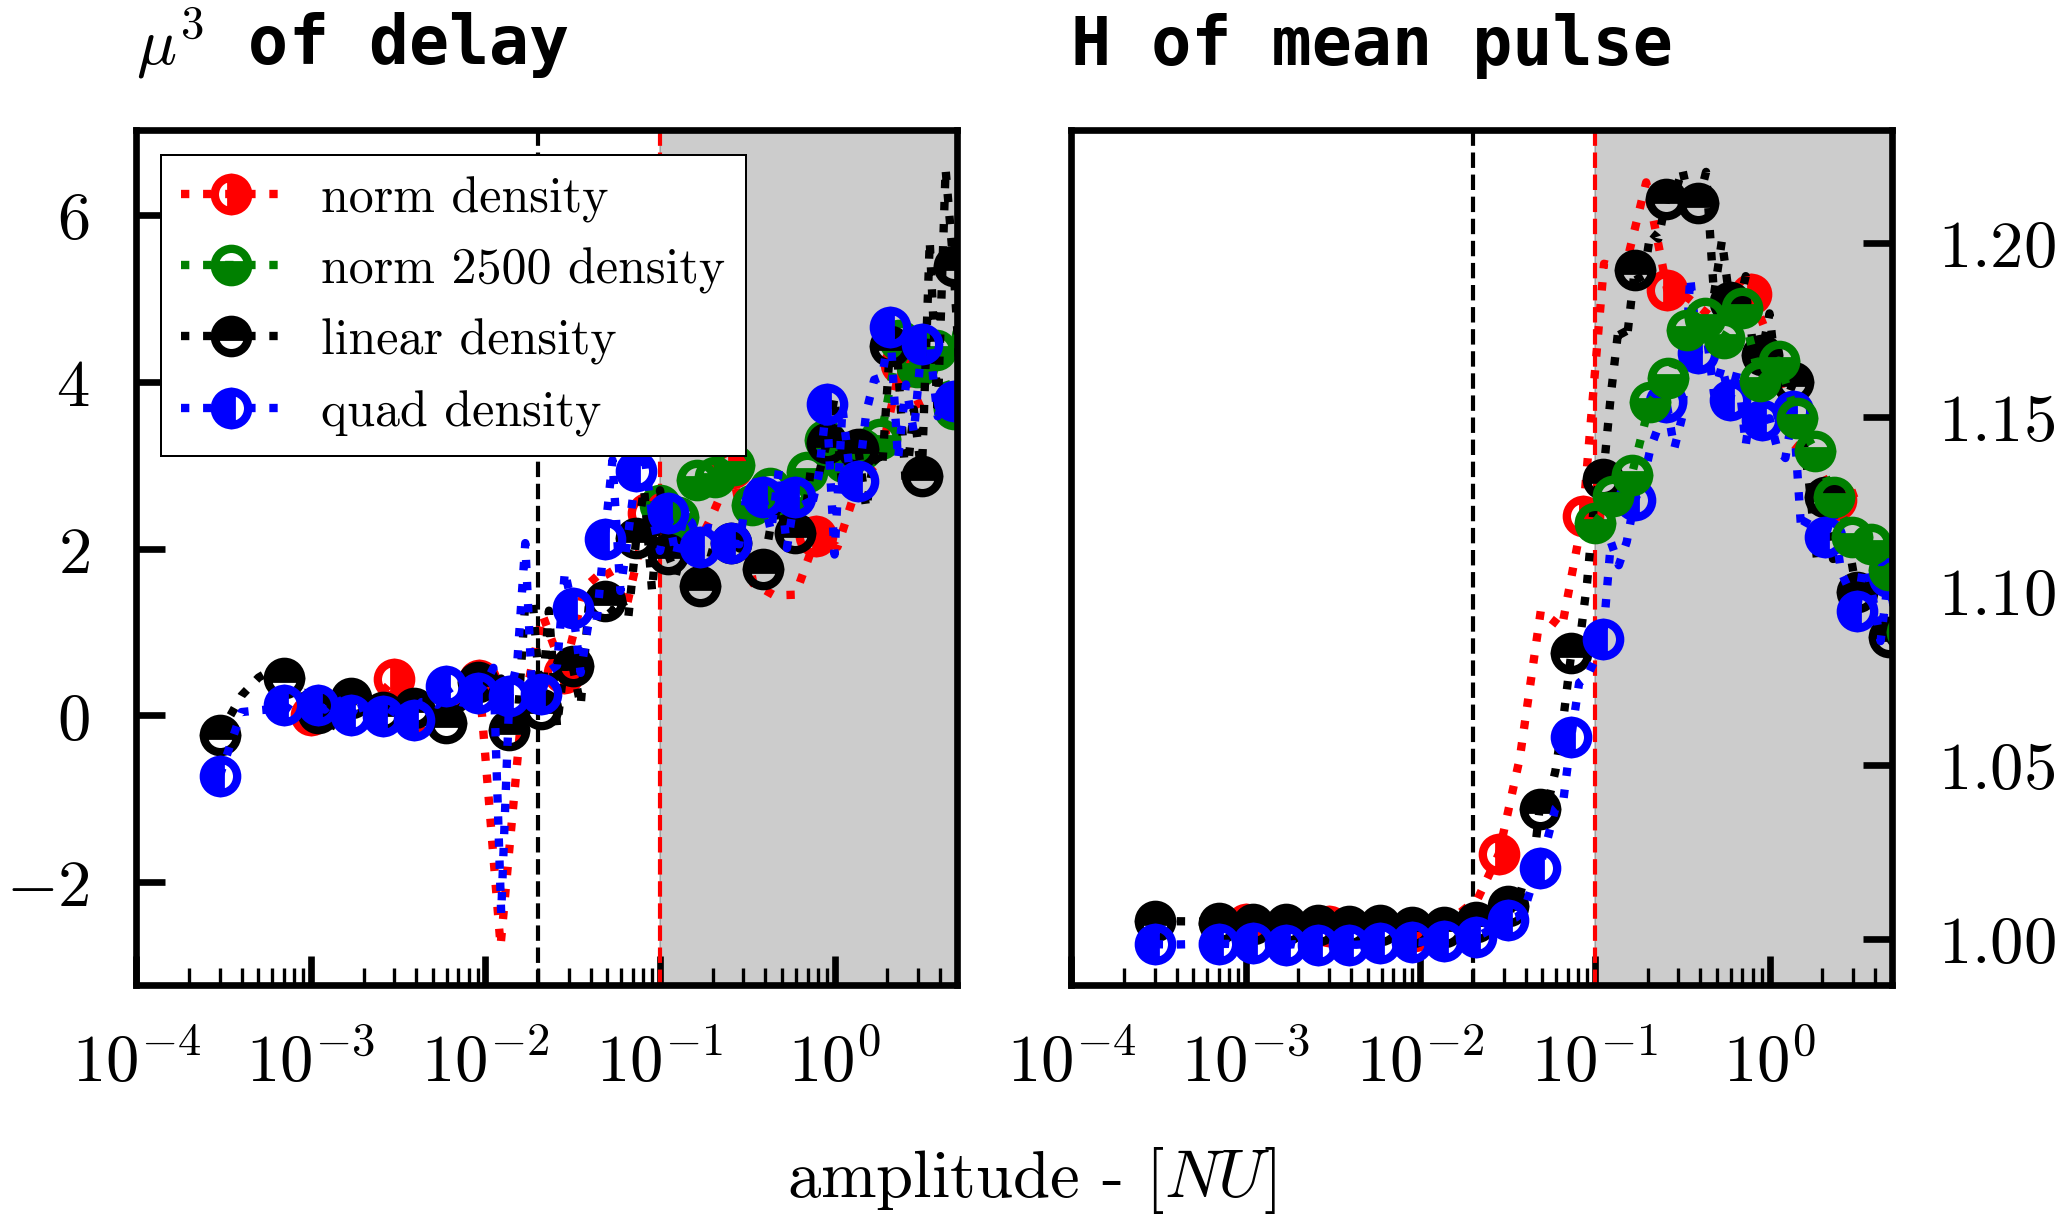
\includegraphics[width=1\linewidth]{./figures/skew_Hyst.png}
        \caption{Here we computed the skewness $\mu^3$ and the hysteresis \textbf{H} of the mean pulse for the previously discussed density profiles. As expected, the skewness of the pulse increases with the profile complexity, while the evolution of hysteresis is even more pronounced. It is important to note that both metrics are significantly influenced by the second critical density value \ref{CRITICAL}, where multiple scatterings become non-negligible.}
        \label{}
    \end{figure}
    The two last metrics seem to be relevant input variables to describe the relative evolution of the pulse shape with respect to the amplitude level. After studying the evolution of the normalized mean pulse shape, we analyzed the statistical properties of the pulse shape to identify relevant metrics for our model.
    \subsection{Statistical Study of Pulse Shape}




    \begin{figure}[H]
        \centering
        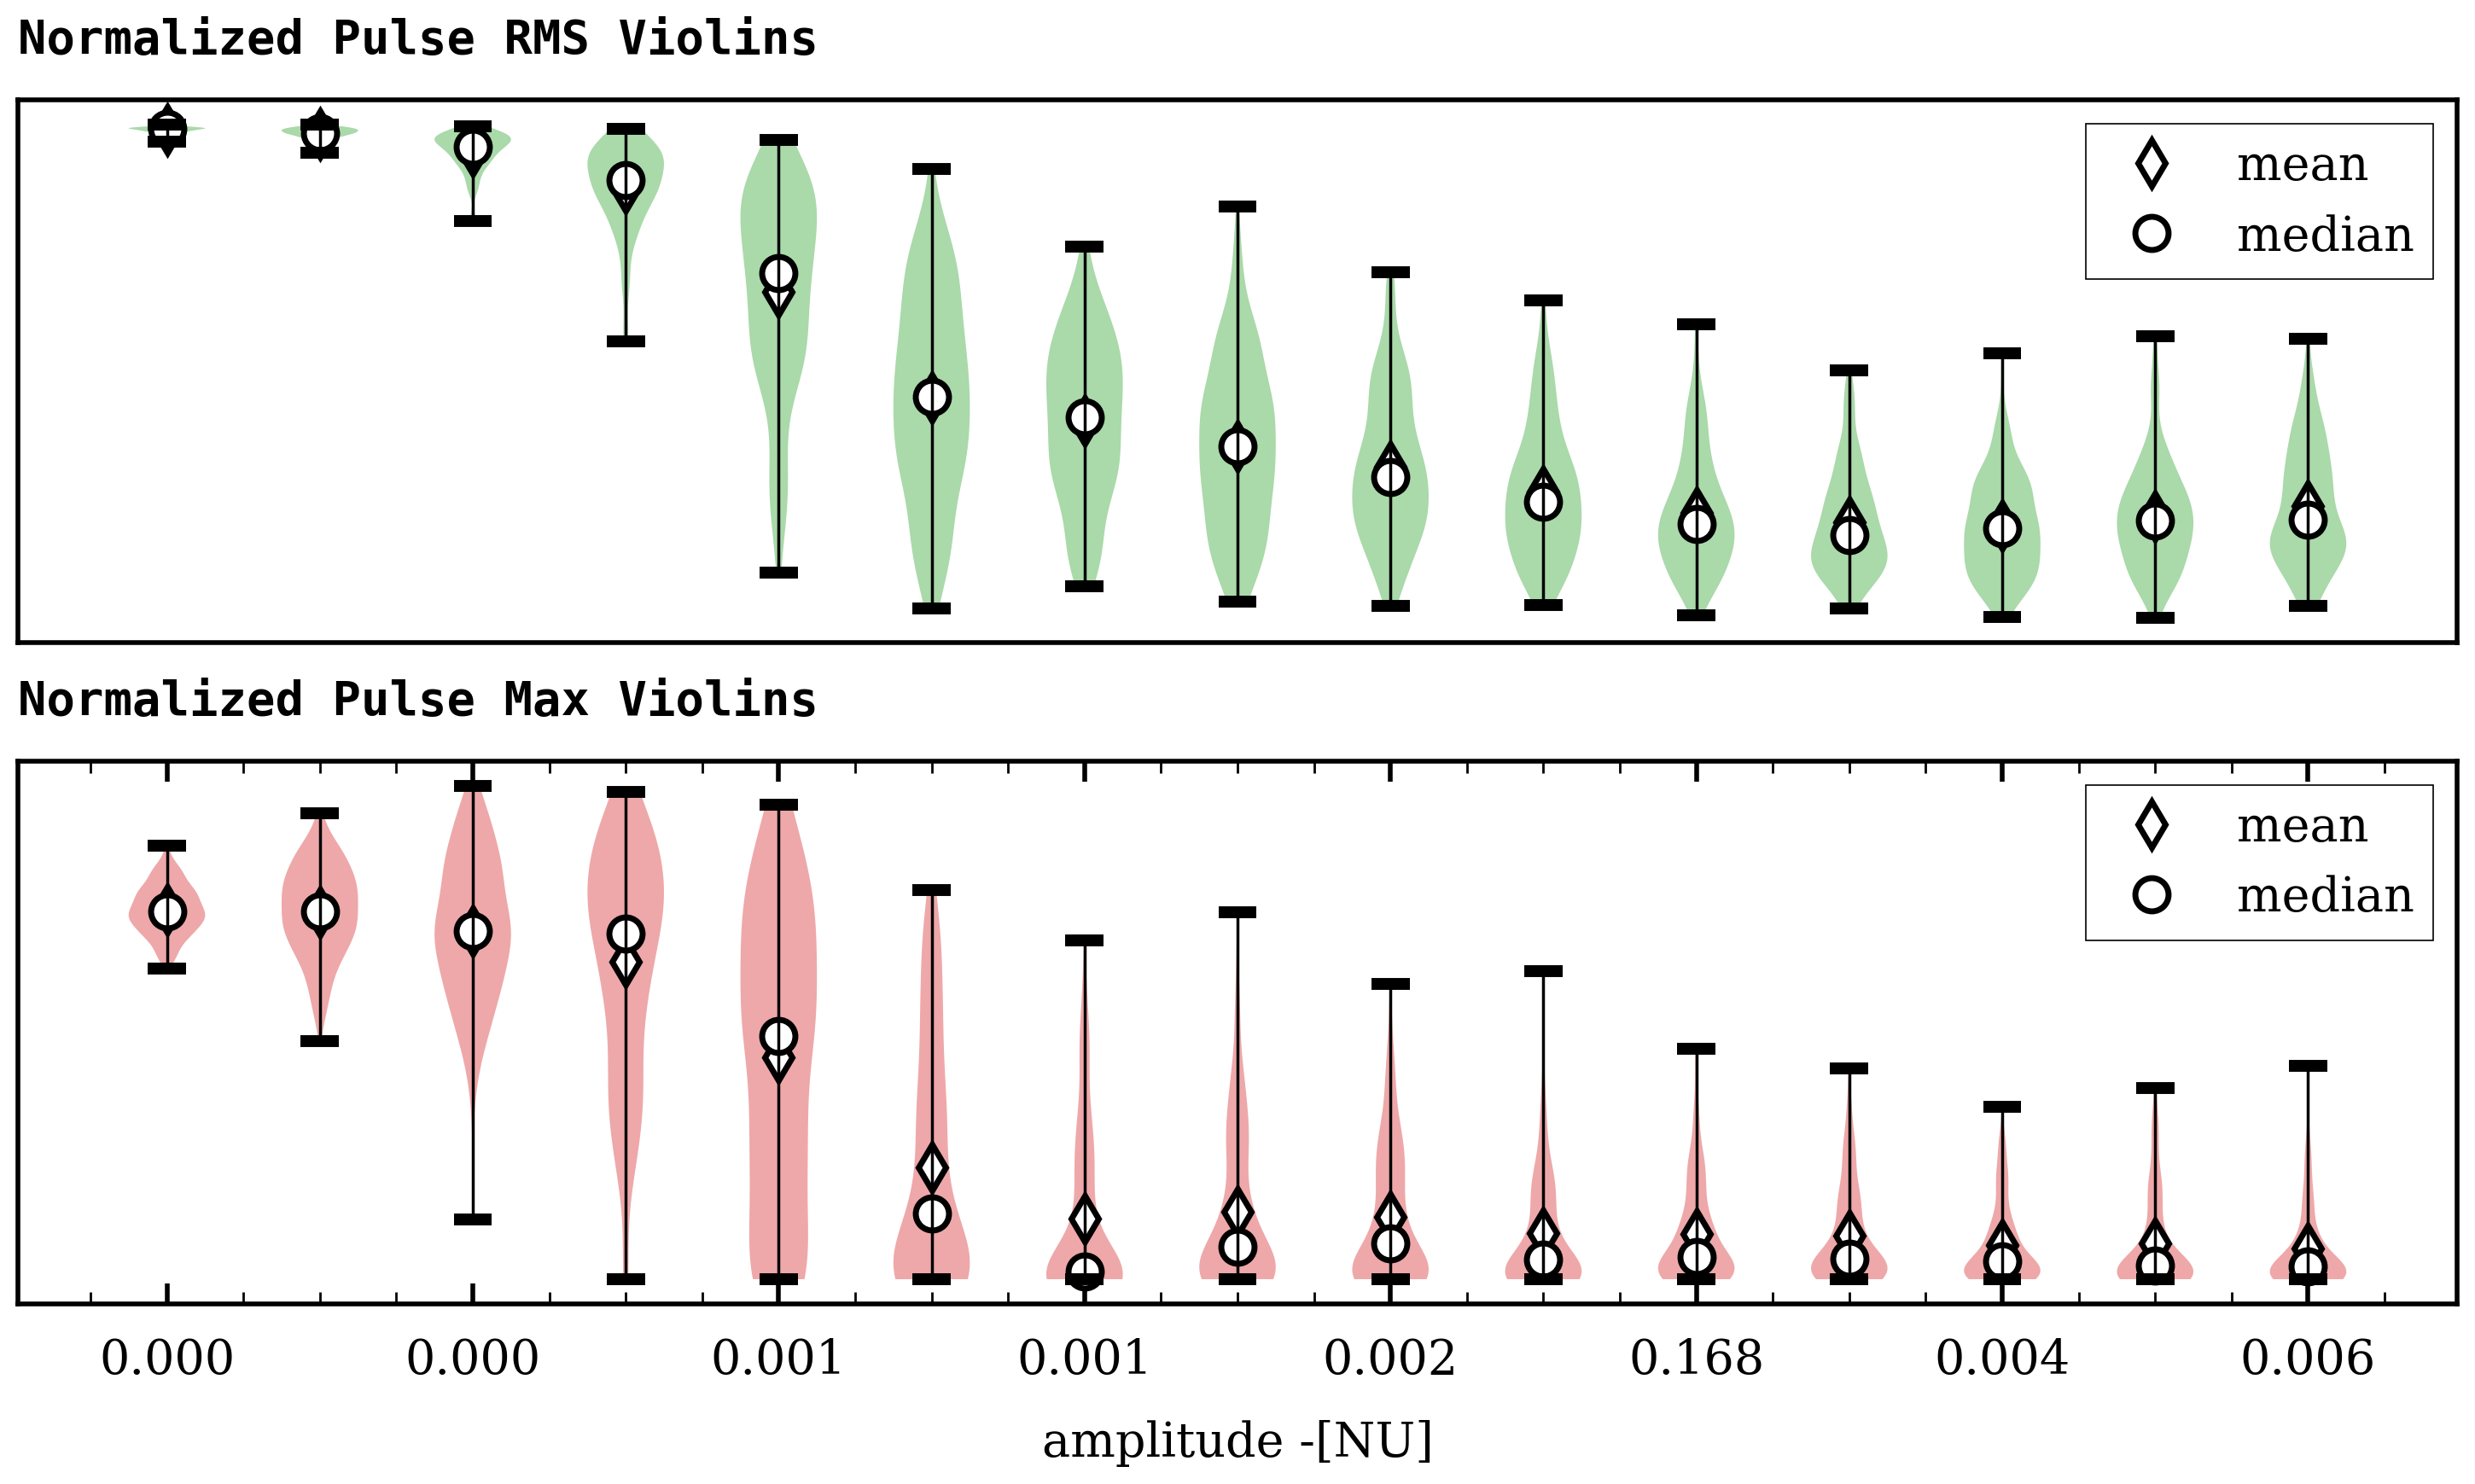
\includegraphics[width=1\linewidth]{./figures/pulse_overview.png}
        \caption{Violin plots of the pulse root mean square (rms), amplitude, and width distributions over perturbation amplitude. The simulations considered a linear density profile background (\textbf{LD}) with a spatially independent $\delta n_0$.}
        \label{fig:barrier}
    \end{figure}The distribution of the pulse RMS and amplitude becomes broader during the transition regime. This broadening is due to the randomness introduced by the perturbations, which persists at large amplitudes, even though the distribution stabilizes. Both the amplitude and RMS of the pulse are highly correlated, reflecting similar dependencies on the amplitude level and characterizing the transition regime between the two critical densities. The pulse width distribution study is more relevant in the Non-Linear regime, where the standard deviation and maximum pulse width evolve smoothly. The mean pulse width, however, remains relatively constant and does not provide significant additional information.

    From this study, several conclusions can be drawn. First, the mean pulse amplitude provides valuable information for characterizing the pulse amplitude distribution. Second, evaluating the pulse standard deviation is somewhat redundant with the amplitude study. Finally, analyzing the pulse width through its standard deviation can yield useful insights, particularly in the full Non-Linear regime (beyond the second critical density). These conclusions were derived from a simple linear density profile; similar trends were observed with the other two density profiles (\textbf{ND}, \textbf{QD}). The only notable difference was a shift in the delay distribution due to the larger vacuum layer when using a quadratic density profile.

    \subsection{Gaussian Fitting of the Pulse}

    One way to assess the deformation of the Gaussian pulse is to track the relative error of the Gaussian fit. This method allows us to study the true Gaussian standard deviation, mean, and amplitude. The following figure shows the relative error of the Gaussian fit and the Gaussian fit itself.
    \begin{figure}[H]
        \centering
        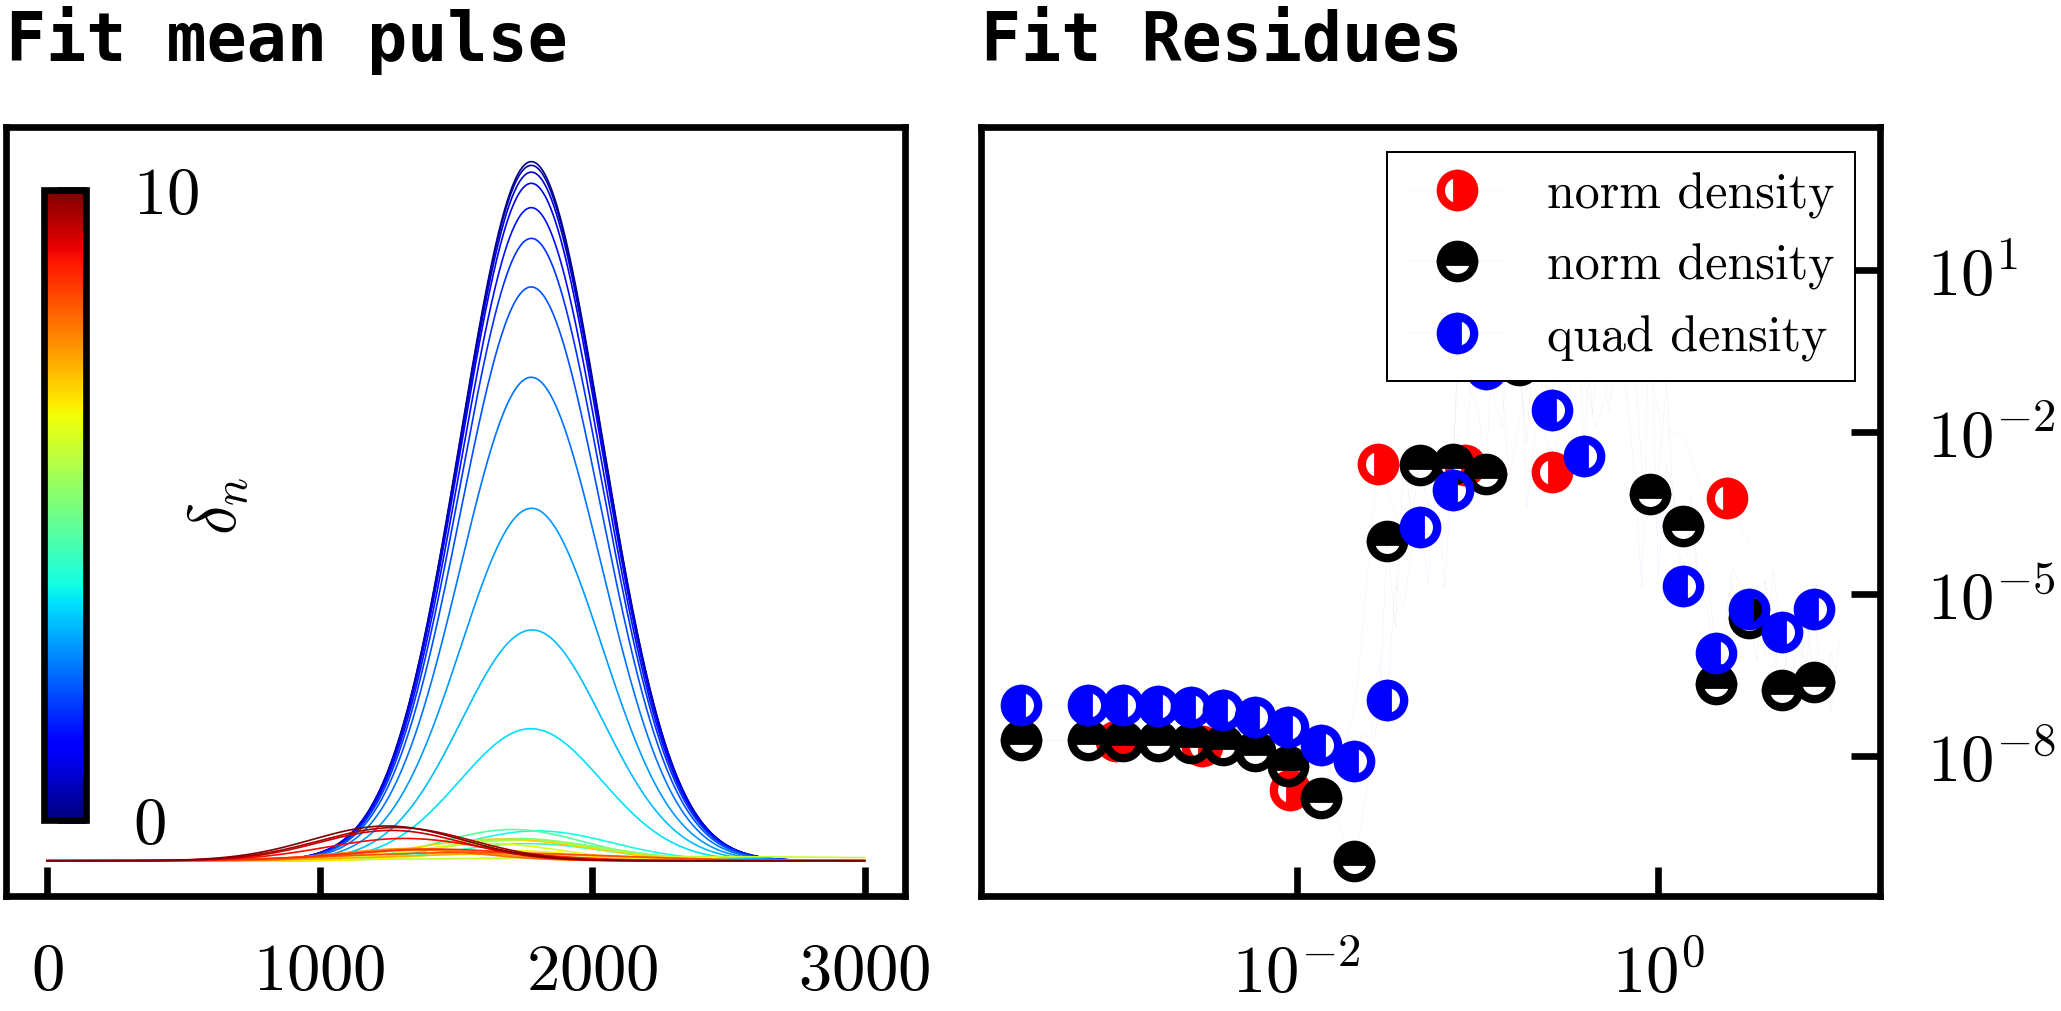
\includegraphics[width=1\linewidth]{./figures/gaussian_fit.png}
        \caption{On the left, the Gaussian fit of the mean pulse is shown for several turbulence amplitudes. On the right, the relative error of the Gaussian fit evolution is plotted, with residuals weighted by the size of the respective pulse amplitude, as a function of turbulence amplitude.}
        \label{}
    \end{figure}
    The residuals are getting large in the transition zone of the pulse shape and seem to decline for very large turbulence. However, we need to find smooth metrics to characterize the transition, rather than relying on pseudo-random metrics, to achieve better predictions in the next part. The Gaussian parameters are also promising candidates and are plotted in the next figure.
    \begin{figure}[H]
        \centering
        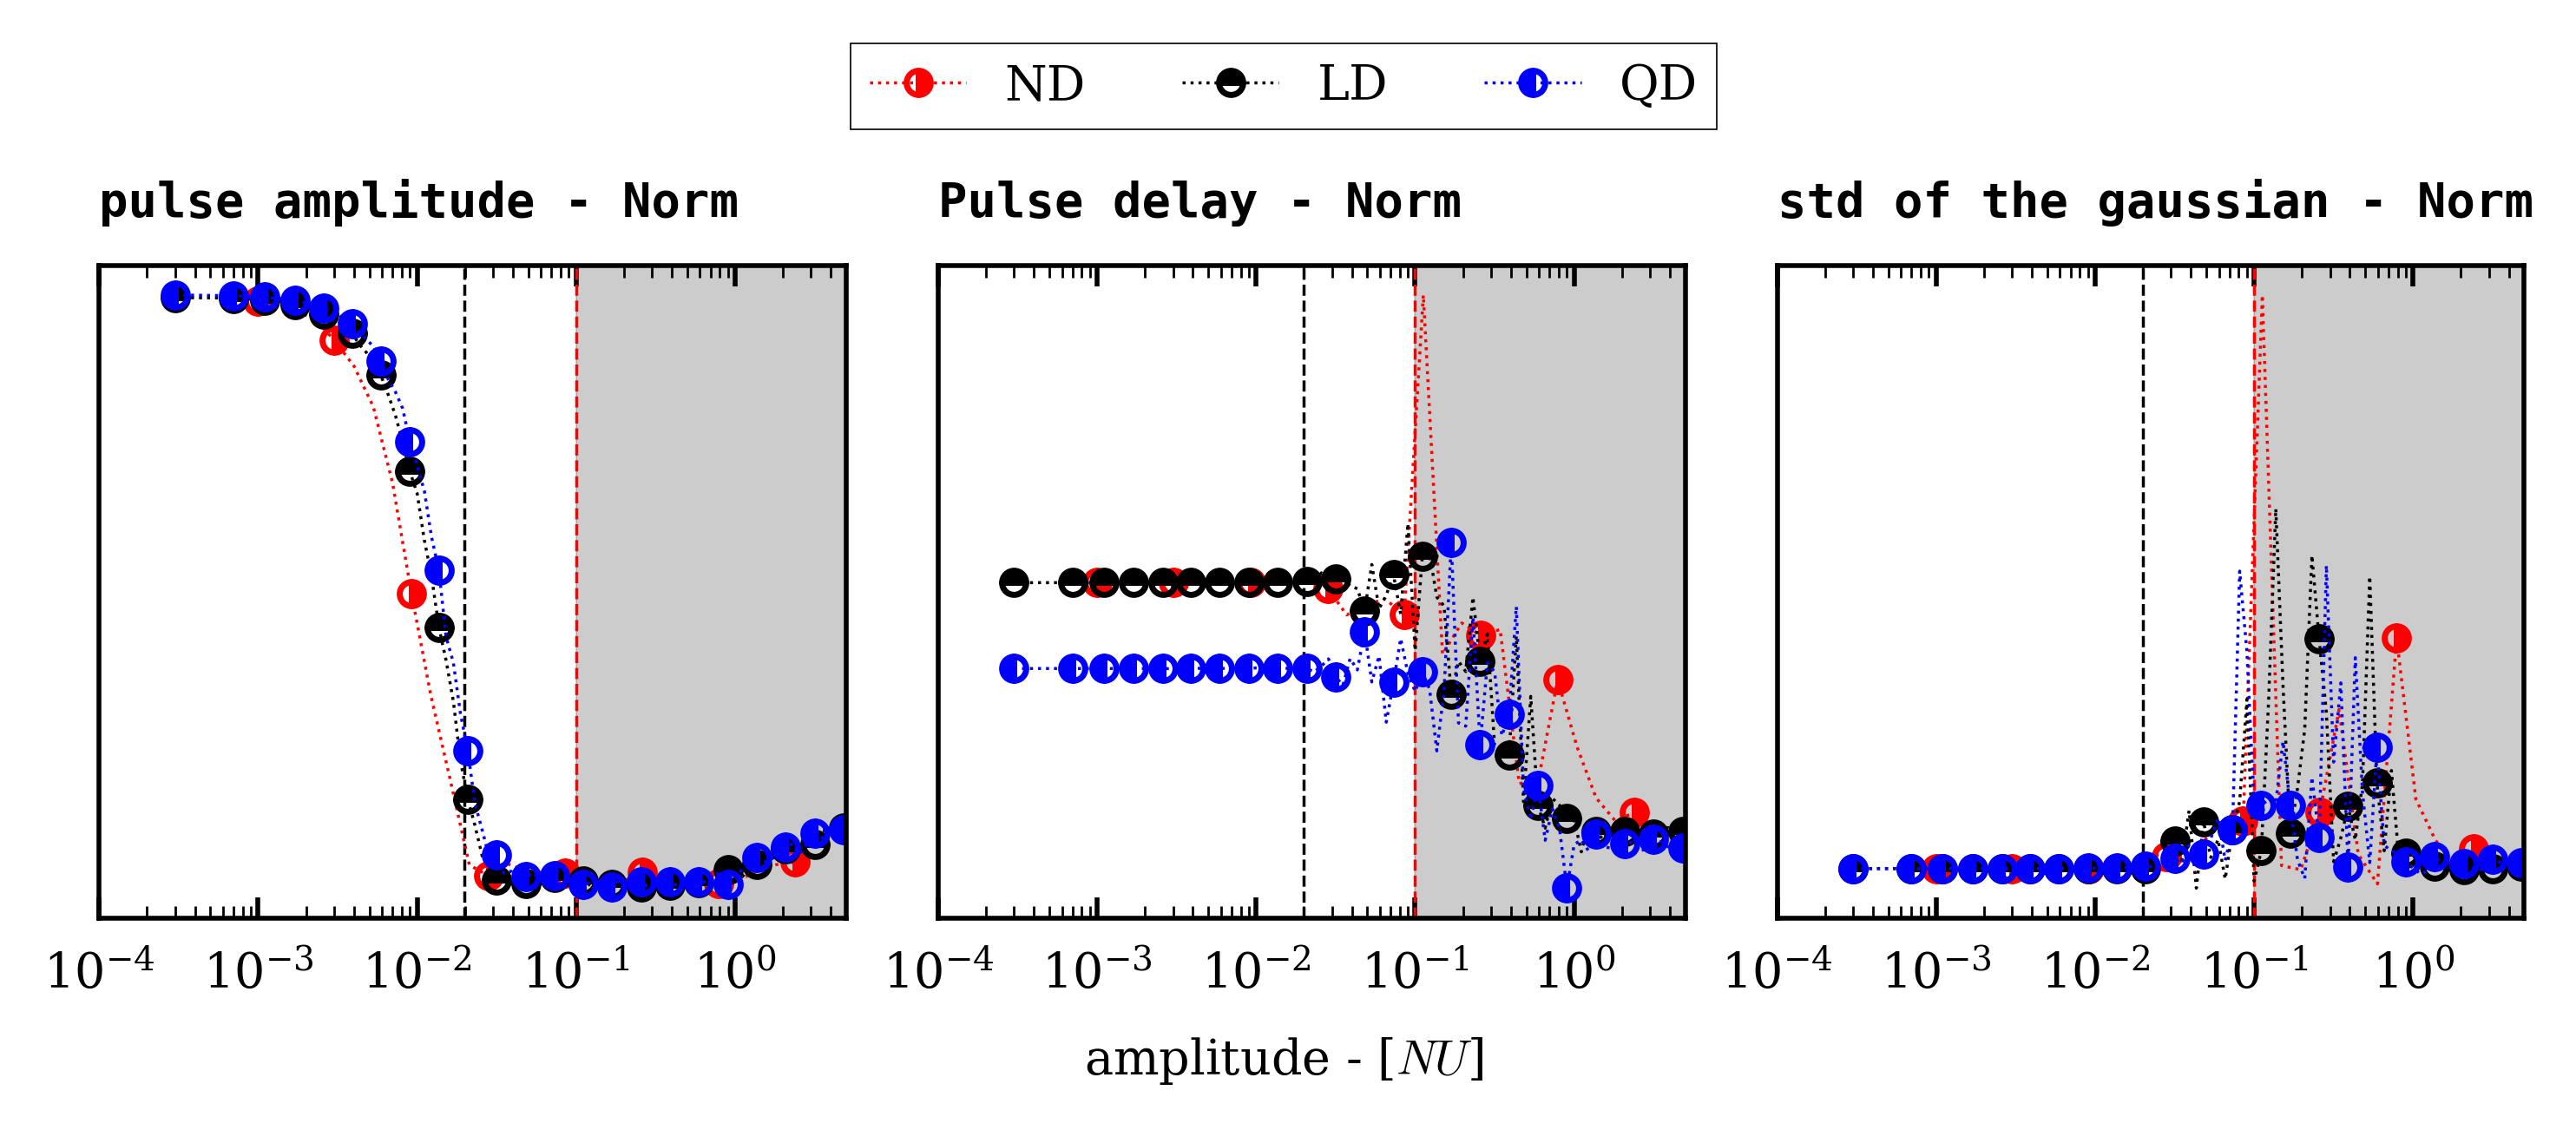
\includegraphics[width=1\linewidth]{./figures/gaussian_Params.pdf}
        \caption{Gaussian fit parameters evolution over the increasing of turbulence amplitude}
        \label{}
    \end{figure}

    Gaussian pulse delay and standard deviation exhibit chaotic behavior during the transition regime, making them less relevant candidates for the next study. However, the Gaussian pulse amplitude shows a relatively smooth behavior, though it reveals a plateau during the nonlinear transition, which might not be ideal. Despite this, at large amplitudes, it captures a similar behavior as the non-Gaussian amplitude, which may be worth studying further in the highly nonlinear regime.

    % \subsection{Detection of Scattered Pulse}

    % Another way to examine the effect of the nonlinear regime on the probing pulse is to study the multiple scattering effects. For instance, the number of secondary spikes could be a good indicator of the nonlinear regime, and the amplitude of these scattered pulses might also be of interest. To achieve this, we need a systematic method for detecting all the spikes. And fit them with a gaussian pulse.  This has been accomplished using the \texttt{SpikeWizard} library, a Python library designed to detect spikes in a signal and to fit peaks with a given function.

    \section{Datasets Building}

    For the two-dimensional datasets, we select the following pulse metrics in addition to the quantilized delay distribution: mean pulse amplitude, standard deviation of delay, mean hysteresis, skewness of the mean pulse, and standard deviation of pulse width. We start by generating a 2D dataset based on a spectral density field. The real field is then obtained using the inverse Fourier transform of the $\delta n(\textbf{k})$ field. For each simulation, we record the pulse signal with and without the turbulence field, using approximately 500 samples. The raw data is processed online on LEONARDO to extract the pulse metrics and delay distribution. This data is saved in a SQL dataset built for this purpose, with simpler Python integrated operations on the data, and then transferred to the SPC computer for further data operations. We follow the same procedure as for the 1D dataset, including standard normalization and the same training/testing split, with the simulation parameters as input and $\delta n_0$, $\tau_0$ as output.
    % - REDUCTION OF BM AND LCX CORR MATRIX
    % - PLOT WITH ALL THE CORR MATRIX
    % - USE SPIKEWIZARD
    % - LCy PARAMS FOR 2D with 1D COMPARISON
    % - 2D MODEL TRAINING
    % - 2D MODEL TESTING (AMP AND TD0)
    % - 2. Histogram of residual
    % - LEVERAGES
    \subsection{Gaussian spectrum of the turbulences}
    The Gaussian spectrum is the simplest way to model turbulence and was used as a first approximation to assess whether the model could integrate dependencies related to different correlation lengths. The parameters used for the 2D simulations with the CUWA code on **LEONARDO** are as follows:
    \setlength{\tabcolsep}{.008\linewidth}
    \begin{table}
        \begin{tabular}{c|c|c|c|c|c}
            \toprule
            \multicolumn{6}{c}{Parameters range}                                                     \\
            \cmidrule{1 -6}
            $\delta n_0$   & $L$ -[cm] & $l_{cx}$ -[cm] & $l_{cy}$ -[cm]  & $\theta$ -[°] & $R$ -[m] \\
            \midrule
            $[1e^{-3}, 1]$ & $[5-18]$  & $\{1, 0.5 \}$  & $\{0.5,2,30 \}$ & [0-10]        & [0.2,5]  \\
            \bottomrule
        \end{tabular}
        \caption{2D simulation parameters range based on Gaussian spectrum}
        \label{Gaussian_table}
    \end{table}

    $\theta$ stands for the incident angle of the probing beam, $R$ the geometry curvature, $l_{cx}$ the typical correlation length of the turbulence in the $x$ direction, and $l_{cy}$ the typical correlation length of the turbulence in the $y$ direction. The $R$ range is chosen to tackle flat and near TCV tokamak geometries. $\theta$ values are dependent on the $R$ range and cannot be too high; indeed, if we consider a high curvature, the incident angle cannot be too high because the probing beam will not be able to reach the cut-off layer, or will be reflected not in the direction of the antenna. This is why we limited ourselves to 10 degrees, with $R = 0.2$ m. In the Gaussian case, the power spectrum of the turbulence is given by the following formula:
    $$
        \delta n(\textbf{k} ) = \delta n_0 \exp\left(-\frac{(k_x l_{cx} k_y l_{cy})^2}{8} + i\Phi(\textbf{k} )\right)
    $$
    This formula will be used to create the first part of the dataset with defined correlation lengths. However, one could argue that the power spectrum of \textbf{TEM} instabilities is not Gaussian.

    \subsection{Power Spectrum of the Turbulences}

    Indeed, the power spectrum of the turbulences provides a more realistic approach to the turbulence profile (give details for each literature measurement of the knee power spectrum). Then explain why the power spectrum is much more complicated to have a continuous one. Introduce the formula of the power spectrum used [cite], and the different parameters used:
    $$
        \rangle\delta n^2 \langle = \frac{1}{1 + \left| \frac{k_x}{W_x} \right|^\gamma + \left| \frac{k_y - k_y^*}{W_y} \right|^\beta}
    $$
    With $W_x$ the $x$ spectral width, $W_y$ the $y$ spectral width, and $k_y^*$ the injection driving scale of the instabilities [CITE]. Note that all the parameters are normalized by $\rho_s$, the ion gyro-radius. This formula has the advantage of not being separable in $x$ and $y$, which is the case in ... [cite].

    \subsubsection{Correlation Length Dependency Study}

    As it is not determined by the power spectrum formula, we have to shift to measured $l_c$ as an input for the model. This is why it is convenient to have a relationship between all the parameters and the correlation length. The expression of $l_{cx,cy}$ can be found using the \textbf{CCF} on many field samples ($s$).

    $$
        r_{xx}(\tau) = \frac{\sum_{s}\left(\tilde{\delta n_s}(x + \tau, y)\right)\left(\tilde{\delta n_s}(x, y)\right)}{\sum_{s}\left(\tilde{\delta n_s}(x, y)\right)^2}
    $$
    With $\tilde{\delta n_s}(x,y) = \delta n_s(x,y) - \bar{\delta n_s}(y)$. The Wiener-Khinchin theorem [CITE] provides another method to compute the correlation length without the need for many samples. Indeed, supposing $k_y$ is constant for the integration, we have for the $x$ correlation length:
    $$
        r_{xx}(\tau) = \int_{-\infty}^{\infty} <\delta n(k_x, k_y)^2> e^{2 \pi k_x \tau} \, dk_x
    $$
    With $r_{xx}$ the autocorrelation function. The correlation length is then defined when $r_{xx}$ reaches the $e^{-1}$ level. Developing the expression of the power spectrum, we have:

    \begin{align}
        r_{x x}(\tau) & = \int_{-\infty}^{\infty} \frac{1}{1 + \vert \frac{k_x}{W_x} \vert^\gamma + \vert \frac{k_y - k_y^*}{W_y}\vert^\beta} e^{2 \pi i k_x \tau} \, dk_x \\
                      & = \int_{-\infty}^{\infty} \frac{e^{2 \pi i k_x \tau}}{1 + \vert \frac{k_x}{W_x C^{1/ \gamma}} \vert^\gamma} \, dk_x
    \end{align}
    From this we can see that the autocorrelation function has a spiked shape, whose width is linearly proportional to:
    $\frac{1}{W_x C^{1/ \gamma}}$

    with $ C = 1 + \left| \frac{k_y - k_y^*}{W_y} \right|^\beta $. The same reasoning can be applied to the \( y \) correlation length, with the same width dependency. This leads to the following dependency:

    $$
        l_{cx} \propto \left(\frac{1}{W_x C^{1/ \gamma}}\right) \, ,\, l_{cy} \propto \left(\frac{1}{W_y Z^{1/ \beta}}\right)
    $$

    With $ Z = 1 + \left| \frac{k_x}{W_x} \right|^\gamma $. For large-scale turbulences like \textbf{TEM}, the spectral width is greater than the wave number since it's known to be a large-scale phenomenon. This leads to $ C \approx 1 $ and $ Z \approx 1 $. We then have:

    $$
        l_{cx} \propto \frac{1}{W_x}  \propto \rho_s \, ,\, l_{cy} \propto \frac{1}{W_y} \propto \rho_s
    $$

    Then we numerically computed the correlation length using the true \textbf{CCF} and Wiener theorem to determine the proportionality constant for both $ x $ and $ y $cases. Thanks to this, we can keep the correlation length as an input for the model, rather than the spectral width, which is more difficult to measure. We try to derive the full expression of the autocorrelation function $r_{xx}(\tau)$ from complex integration of the function $\frac{e^{2\pi ix \tau}}{1 + x^\gamma}$ over the contour $\gamma$ defined as the $R$ radius positive hemi-circle in the complex plane, This leads to a complex relation of the form $$r_{x x}(\tau) \propto \sum_{res} e^{\sin(\theta_i)}sin(\theta i) $$ We did not suceed inverting this expression to isolate $\tau$ even with deep study of approximations near the poles.
\end{multicols}
\noindent
\rule{\linewidth}{0.4pt}

\begin{figure}[H]
    \centering
    \hspace*{-0cm}\includegraphics[width=1.\linewidth]{./figures/CCF_Wiener.pdf}
    \caption{On the left, the $r_{xx}$ values computed using both the \textbf{CCF} and Wiener Theorem are plotted for various $\rho_s$. On the right, a linear fit is shown between the correlation length and the ion gyro-radius. A similar study was conducted for the $y$ correlation length dependency. Note that for generating the $\rangle \delta n \langle^2$ field, the following parameters were used: $D = 6.3 \times 10^{-3} (\frac{\rho}{L})^2$, $W_x = \frac{3.71}{\rho_s}$, $W_y = \frac{4}{\rho_s}$, $\beta = 2.88$, $\gamma = 3.14$, and $k_y^* = \frac{0.1}{\rho_s}$. The $l_{cx}$ and $l_{cy}$ calibration (see fig: \ref{Wiener}) was performed using these values as referenced in [CITE].}
    \label{Wiener}
\end{figure}
\begin{multicols}{2}
    The correlation length fit of the Wiener theorem appears to have the smallest residuals and leads to the same results as the \textbf{CCF} method, without computing too many samples. We can then obtain the following formula for the correlation lengths, which should lead to the same turbulence structures as the Gaussian spectrum (see Fig: \ref{fig:density_field}):
    \begin{equation*}
        \begin{cases}
            lc_x = (1.19 \pm 0.02) \rho_s + (0.0012 \pm 0.0001) \\
            lc_y = (1.35 \pm 0.03) \rho_s + (0.0015 \pm 0.0001) \\
        \end{cases}
        \label{eq:}
    \end{equation*}
    We can then use these formulas to compute the correlation length for the 2D datasets, which will be input parameters for our model, and then use the power spectrum formula to compute the $\delta n(\textbf{k} )$ field.

    \setlength{\tabcolsep}{.02\linewidth}

    \begin{table}[H]
        \begin{tabular}{ccccc}
            \toprule
            \multicolumn{5}{c}{Parameters range}                                         \\
            \cmidrule{1 -5}
            $\delta n_0$   & $L$ -[cm] & $\rho_s$-[m]         & $\theta$ -[°] & $R$ -[m] \\
            \midrule
            $[1e^{-3}, 1]$ & $[5,18]$  & $[2e^{-3}, 2e^{-2}]$ & [0-10]        & [0.2,5]  \\
            \bottomrule
        \end{tabular}
        \caption{2D simulation parameters range based on Power spectrum, the value of $\rho_s$ are choosen to be included in the range of the gaussian dataset values of $l_{cx}$ amd $l_{cy}$. }
        \label{Power_table}
    \end{table}


    \begin{figure}[H]
        \centering
        \includegraphics[width=1\linewidth]{figures/field_power.pdf}
        \caption{Comparison of the turbulence fields for $\rho_s = 8 \times 10^{-3}$ using the corresponding correlation lengths in the Gaussian spectrum. A linear-dependent turbulence profile was chosen with $\delta n_0(x) = \delta n_0 \frac{x}{L}$. The selected plotting area is a (3 cm x 10 cm) rectangle that includes both the cut-off layer and the vacuum layer in a slab geometry.}
        \label{fig:density_field}
    \end{figure}

    In Fig.\ref{fig}, we can clearly observe the same structure of the turbulence field for both spectral approaches, indicating that our initial Gaussian approximation is quite relevant. This relevance not only validates our approach but also suggests that it will significantly enhance our model's ability to generalize its predictions across various turbulence scenarios. Consequently, we will retain this valuable and detailed information for training purposes, ensuring a robust foundation for the model.

    \subsection{Data Scanning}

    For the first part of the training, to ensure a homogeneous data distribution, we chose data points on a defined grid. To refine the model, we then used some random uniformly sampled (logarithmically for $\delta n_0$) data points within the range of the study. To check if the reached distribution is quite homogeneous for the training, we can plot the distribution of the data points in the parameter space and see if the data points are well distributed. This is illustrated in the following figure.

    \begin{figure}[H]
        \centering
        \includegraphics[width=1\linewidth]{./figures/polar_param.pdf}
        \caption{Polar distribution of data points in the parameter space for training. This distribution is evaluated for homogeneity across different parameters to ensure comprehensive coverage of the parameter space. The circle represents the parameter range as described in Table \ref{Power_table} and Table \ref{Gaussian_table}, while the radial value indicates the parameter distribution value. Data points from the power spectrum datasets are shown in blue, and those from the Gaussian spectrum datasets are shown in red.}
        \label{params_distr}
    \end{figure}
    The figure shows that the data points are quite well distributed in the parameter space. One observation is that the $R$ distribution is concentrated near 0 because we chose to plot the curvature $\frac{1}{R}$ rather than the true radius distribution. To account for flat geometries, we introduced an $R = 1000$ value in the datasets, which could have disrupted the normalization process. Additionally, the $l_{cy}$ distribution is unevenly distributed since we also introduced high values of $l_{cy}$ to mimic the 1-dimensional case. Before training, we followed the same procedure as for the 1D datasets, with standard normalization, and used the same training/testing split, with simulation parameters as input along with the previous metrics and $\delta n_0$, $\tau_0$ as output.

    \section{Results}

    The model was trained on the 2D datasets, maintaining the same structure as the 1D model (which was found to be quite robust for handling nonlinearities). The same hyperparameters were used for this study (see Table \ref{Hyperparameters}). The only difference is the number of input data variables, which complicates our model.

    \subsection{Global Performance}

    The model achieved an $R^2$ score of 0.92 for the Gaussian testing set and 0.89 for the power spectrum testing set. These are quite reasonable results, even considering the logarithmic dependency of $\delta n_0$. For comparison, a deep neural network was trained in parallel with the same dataset. This network had 5 layers with (256, 128, 64, 32, 2) neurons in each layer with sigmoid activation. This more complex model achieved a poor $R^2$ score of 0.3, which is significantly below our model's performance. To gain a better overview, we can use the same principle as in Figure ??, comparing the residuals of the model for each parameter value in the testing set. This is illustrated in the fig (3.9).{Here we plot the mean residuals for each parameter value. The residuals for the Gaussian datasets are shown in blue, while those for the power spectrum datasets are in red.
            The model shows a notable improvement over the 1D model, with a mean residual of 0.25. This is ten times smaller than the residuals observed with the 1D model applied to the 2D-shifted datasets. The residuals are generally well-distributed across all simulation parameters.
            However, there are some observations to note: The residuals for the $R$ parameter tend to be concentrated at lower values, which results from the $\frac{1}{R}$ transformation. Additionally, the residuals for the $\theta$ parameter are higher at larger $\theta$ values. This makes sense, as handling higher $\theta$ cases is more challenging.
            Despite these variations, the residuals for both datasets are quite similar in their mean values. This consistency suggests that the model generalizes well across different types of turbulence spectra.}
\end{multicols}
\rule{\linewidth}{0.4pt}

\begin{figure}[H]
    \centering
    \includegraphics[width = \linewidth]{./figures/polar_res.pdf}
    \caption{Here we plot the mean residuals for every value of every parameter, in blue filled we got the residuals for the gaussian datasets, and in red the residuals for the power spectrum datasets. }
\end{figure}

\begin{multicols}{2}

    \subsection{Comparison of the Prediction with Other Models}

    For the previous study, the datasets contained several parameters implying a 2D geometry. However, to compare our model with the 1D model and the analytical model, we need to build a final comparison dataset. To ensure clear results, we will fix the parameters $l_{cy}$, $R$, $\theta$, $L$, and $l_{cx}$ to the same values for both the 1D and 2D models. This allows us to examine if our model can handle the simpler 1D case. We will study the dependency of predicted $\delta n_0$ on true $\delta n_0$, which provides a general perspective on $\text{rms}(\tau)$ over $\delta n_0$. Additionally, for the 1D analytical model, we have the equation $< \tau > = \tau_0$.

    \subsubsection{Mean Delay Study}

    In the nonlinear regime, the previous assumption $< \tau > = \tau_0$ may be invalid. Our model should be able to address this case. To investigate this effect, we will study the dependency of $\tau_0$ on $\delta n_0$. In the nonlinear regime, the probability of a shift in the cut-off layer being positive or negative is not equal. Specifically, there is a higher probability of a negative shift than a positive shift. Consider a given $n_c$ and $\delta x$ value. We will use a 1D model with a density variation probability density function (PDF) that does not account for spatial correlation length:

    $$
        p(\delta n, x) = \frac{1}{\sqrt{2 \pi \sigma^2}} e^{-\frac{\delta n^2}{2\sigma^2}}
    $$

    where $\sigma \propto \delta n_0$. We are interested in the first-hitting position, which is a sub-branch of survival stochastic analysis. The probability of survival $S(x)$ (i.e., the probability that the density does not reach the $\delta n_c$ value before $x$) is given by the critical density variation $\delta n_c = n_c \frac{L - x}{\sigma}$. The goal is to show that the probability of the first hitting position decreases with $x$.

    To include the correlation length of the instabilities field, we must account for it in the survival probability calculation. If not, the survival probability will be simply zero. For simplicity, we will discretize the interval of study $[0, x]$ with $\left\lfloor \frac{x}{l_{cx}} \right\rfloor$ points. This approximation assumes that every point in each interval of length $l_{cx}$ has the same probability of survival, equivalent to a step approximation. The probability of having a value smaller than $\delta n_c$ at a specific point $i$ is given by the following formula:
    \begin{align*}
        P(\delta n_c, ia) & = \int_{-\infty}^{\delta n_c} p(\delta n, ia) \, d\delta n                         \\
                          & = \frac{1}{2}\left(1 + \text{erf}\left(\frac{\delta n_c(ia)}{\sigma}\right)\right) \\
    \end{align*}
    The survival probability at point  $x = ia$ is then given by the following formula :
    \begin{align*}
        S(ia) & = \prod_{j=0}^{i} P(\delta n_c, j*a) \\
    \end{align*}
    The probability that the first hitting position is at \( x = il_{cx} \) is then given by

    \[ F(il_{cx}) = S(il_{cx})P(il_{cx}). \]

    The goal of this study is to show that \( F(x) \) has a maximum located before the original cut-off position. To demonstrate this, we computed numerically the value of \( S(il_{cx}) \). From this computation, we find an interesting approximation of the survival function. For a Gaussian (shifted) process, the numerical results show that the survival function can be approximated by:

    \[ S(x) \approx \frac{1}{2} \left[1 + \text{erf}\left(\frac{x - \mu}{\sigma \sqrt{2}}\right)\right], \]

    where \( \text{erf} \) is the error function, \( \mu \) is the mean of the distribution, and \( \sigma \) is the standard deviation.

    \begin{equation}\label{survival}
        S(x) \approx \frac{1}{2} + \frac{1}{2}\text{erf}\left(\frac{L - x- a(l_cx, L, \sigma)}{b(l_cx, L, \sigma)} \right)
    \end{equation}
    With \( a(l_{cx}, L, \sigma) \) the characteristic shift and \( b(l_{cx}, L, \sigma) \) a characteristic width, this approximation is the probability to remain below the critical value at a position \( x - a(l_{cx}, L, \sigma) \) with a modified distribution of instability amplitudes \( \mathcal{N}(0, b(l_{cx}, L, \sigma)) \). We can note that this result is very close to the survival function of a Brownian process. Considering an absorption point \( x_c \), the first hitting time method used in this kind of problem was not applied here due to the linear shift of the Gaussian distribution, which was very difficult to handle because we need to consider a moving absorption point to make the parallelism.

    \begin{figure}[H]
        \centering
        \hspace{-1.2cm}\includegraphics[width = 1.13\linewidth]{./figures/First_Hitting.pdf}
        \label{fig:FHP}
        \caption{Here we plot the numerical calculation of $F(x)$ the First timeHitting probability (\textbf{FHP}) for numerous $\sigma$ in plain line  and the approximated formula \eqref{survival} in dotted line. . For this simulation we used $L = 10$cm and $l_{cx} = 0.1$cm, and for the approximated formula we used $a = 2.1 \sigma^{1.5}L$ and $b = .36\sigma^{0.8} L$, we did not study the dependancy over $l_{cx}$ but this one is clearly in the power and the coefficient of $a$ and $b$.}
    \end{figure}One can remark that the \textbf{FHP} is shifted to values before \( L \) as \( \sigma \) increases, which explains the radial external shift of the cut-off with the increasing amplitude of turbulences. Indeed, we can assume a linear dependency between \( \sigma \) and \( \delta n_0 \). This shift will result in a difference between \( \langle \tau \rangle \) and \( \tau_0 \), with \( \tau_0 \) remaining constant and \( \langle \tau \rangle \) decreasing. We already know that the linear model is not able to capture this precision—what about the new models?
    \begin{figure}[H]
        \centering
        \hspace*{-1.3cm}\includegraphics[width = 1.14\linewidth]{./figures/Mean_delay.pdf}
        \caption{Here we plots the linear and the 1d, 2d model prediction for $\tau_0$ over the $\langle \tau \rangle$. The plot bellow ist the evolution of the residuals between the predicted $\tau_0$ and the real one over the amplitudes of the turbulences. On the left plot the cumulative function of the residuals. This verification has been done on 2 dimensional dataset with a curvature $\frac{1}{R} = 4$, this allows us to see the difference of efficiency between the 1D and 2D model}
        \label{fig:mean_delay}
    \end{figure}

    Here we can see that the 1D model and the 2D model, built on the same architecture, have very different prediction and only the final 2 dimensional model is able to predict a constant \(\tau_0\) independently of the changing delay distribution. This was intended since the models are trained on a constant \(\tau_0\) that depends only on \(L\), \(R\), and \(\theta\). The residuals evolution highlights that for high amplitude the linear and the 1D model do not have good predictions for this geometry, thanks the DF we can see that this prediction is oftenly higher than real value. For the 2D model the residuals presents no assymetric spread or too high value.

    \subsubsection{Amplitude prediction study}

    The first thing we did was comparing the efficiency of all the models we built with the \((\delta n_0, \delta n_0^{\text{pred}})\) comparison. This involves evaluating the results of the residuals, which show that our latest model performs much better than the others. The more the points deviate from the identity line, the worse the model's performance.

    \begin{figure}[H]
        \centering
        \hspace*{-1.3cm}\includegraphics[width = 1.1\linewidth]{./figures/amplitude.pdf}
        \label{}
        \caption{Plot of the linear and the 1d, 2d model prediction for $\delta n_0$ over  $\delta n_0^{\text{true}}$. The simulation set-up is the same as the fig \ref{fig:mean_delay}. In filled blue the 95 \% Confidence interval of the 2d model}
    \end{figure}

    Here some interesting observations can be made. The linear model is not able to predict the amplitude of the turbulence for high turbulence amplitudes, which is not surprising given the complexity of the problem. Regarding the 1D model, the accuracy collapses even with the shift of the delay distribution. We can also note that, even in the linear regime, its performance is quite poor.

    The 2D model, however, is able to predict the amplitude of the turbulence with a high degree of accuracy. Especially in the non-linear regime, there is no saturation of the prediction.

    The study of the residuals leads to the same conclusions as before: the 2D model residuals are well-distributed and have a low value, while the 1D model residuals and the analytical model have wider range of possible, with a cumulative function (DF) broader than the 2d one.
    \subsubsection{Standard deviation of delay}

    As explained with \ref{fig:std_delay}, the RMS of the delay distribution should decrease at high amplitude from \(\delta n_{c_1}\). This decrease is not well addressed by the linear model (the next order of the step model development needs to be studied), or at least not correctly (see the third-order development of the linear model). The previous model should present better results considering the residuals of the predictions.

    \begin{figure}[H]
        \centering
        \hspace*{-0.2cm}\includegraphics[width = 1.12\linewidth]{./figures/Std_delay.pdf}
        \label{}
        \caption{Plot of $\sigma_{\tau_d}$ over the linear and the 1d, 2d model prediction for $\delta n_0$. The simulation set-up is the same as the fig \ref{fig:mean_delay}. This plot was made to make the parallel with the fig \ref{fig:std_delay}, to see if the model is able to predict the characteristic saturation of the $\sigma_{\tau_d}$ over the $\delta n_0$. The residuals are calculated relatively to the error on the predicted amplitude. In filled blue the 95 \% Confidence interval of the 2D model}
    \end{figure}

    As we saw in the fig \ref{fig:std_delay}, the linear model is not able to predict the saturation of the delay distribution, and predict a linear dependancy of $\sigma_{\tau_d}$ over the turbulences amplitudes. The 1D and 2D model are able to predict the saturation of the delay distribution, with a wider ranger of amplitude for the last one. However one can note that in linear regime both model struggle to tackle the linear dependancy over the amplitude of the turbulences. A good solution might be to adapt the model after a first prediction of the amplitude by the 2d, if the predicted amplitude is in the linear regime, then you should switch to linear model for a better prediction.

    \subsection{Results on experimental datasets}

    A demonstration of our final model was done on one experimental dataset acquired from the TCV diagnostics. To obtain coherent results, we had to shift the experimental dataset's distribution of delay to match the training dataset. This constant shift is due to the geometry of the probing method, which involves a different void layer. This process will be necessary for future studies. One solution is to have a consistent dataset with the same range of data as our training datasets (see table PUT), or to train the model on another dataset specific to the geometry and diagnostic method used (see the code of the model HERE).

    \chapter{Conclusion and Discussion}

    In this report, we first detailed the origin of one predominant mode of transport in the TCV, the \textbf{TEM} mode, and how it can induce uncontrolled radial transport through resonant interaction with trapped electrons, causing trouble for plasma confinement. We then used a 1D model (proposed by Krutkin) to gain initial insights into the turbulence regime and to assess the relevance of the linear model.

    We then moved on to the analysis of a 1-dimensional dataset with a study of delay characteristics, checking if the nonlinear regime could be handled by the proposed model structure. For the 1-dimensional dataset, the results were encouraging, but when applied to a 2-dimensional dataset, the model lacked sufficient information to properly account for curvature, incidence angle, and multiple scattering effects.

    A more general 2D model was proposed, providing better handling of nonlinear effects emerging from this additional dimension. The data used came from large CUWA code simulations and included more metrics than the 1-dimensional dataset, carefully chosen to provide the best overview of the phenomena at stake. The datasets for training were built around the instability spectrum considerations, involving studies of both the power and Gaussian spectra of \textbf{TEM}. The residuals of the predictions were studied and characterized for every simulation parameter, leading to homogeneous results regardless of the parameter values. Finally, the model predictions were tested on several physical aspects of the problem, including the shifted cut-off handling and the decrease in the rms of the delay distribution.

    These results are significantly better than those previously achieved for turbulence characterization at this level of turbulence amplitude. It is important to note that our model is built on the assumption that we have sufficient insight into the turbulence characteristics, such as the correlation lengths, which can be determined through other diagnostic methods (Doppler Reflectometry Method and Thomson Scattering). If future users of this model lack this insight, they can construct a reduced model by dropping any metrics they do not have. It should be highlighted that the delay distribution and pulse characteristics (at least the standard deviation and quantiles for the delay distribution) are necessary for obtaining meaningful results with this model.

    One might question why we did not use the computational capacity of \textbf{LEONARDO} to build a larger neural network or fine-tune an existing regression neural network. The simple answer is the project's budget and the inference time required. We needed a fast and straightforward model with low inference time on a simple GPU to potentially implement real-time data analysis for plasma control.

    \chapter*{Acknowledgments}

    The author wishes to thank Dr. Oleg Krutkin for his supervision, the instructive discussions for building the final model, and for the careful reading of the manuscript. Many thanks to CINECA clusters and their support during the course of this work, which was crucial for this work performed on a 36-core Xeon cluster.

    This project was carried out within the framework of a master internship under the supervision of the \textit{Ecole Normale Supérieure} through Pr. Jean-François Allemand, who showed great interest in this project. This project was supported by The EUROfusion Consortium and received funding from the FUSEnet organization, the EPFL exchange program, and the Swiss Plasma Center.

    Finally, I need to thank the SPC community for their kindness in listening to my issues and considerations and for the positive atmosphere that prevails in the center.

    \nocite{*}
    \printbibliography
\end{multicols}


\end{document}